\documentclass[12pt,a4paper,oneside]{report}
\usepackage[T1]{fontenc}
\usepackage[utf8]{inputenc}
\usepackage{mathptmx}
\usepackage{textcomp}
\usepackage[a4paper,left=2.8cm,right=2.5cm,top=2.5cm,bottom=2.5cm]{geometry}
\usepackage{graphicx,booktabs,tabularx,array,amsmath,setspace,enumitem,float}
\usepackage[labelfont=bf,labelsep=period,font=small]{caption}
\usepackage{titlesec,tocloft,fancyhdr}
\usepackage[hidelinks]{hyperref}
\setstretch{1.3}
\setlength{\parindent}{0pt}
\setlength{\emergencystretch}{2em}
\frenchspacing
\usepackage[section]{placeins}
\usepackage{xcolor}
\definecolor{titlegreen}{HTML}{EEF8EE}
\setlength{\parskip}{6pt}
\graphicspath{{figures/}}
\renewcommand{\thefigure}{\thechapter.\arabic{figure}}
\renewcommand{\thetable}{\thechapter.\arabic{table}}
\captionsetup[table]{position=above,skip=4pt}
\renewcommand{\tabularxcolumn}[1]{p{#1}}
% chapter and section headings in the institute style
\titleformat{\chapter}[display]{\centering\bfseries}{\large CHAPTER \thechapter}{8pt}{\LARGE\MakeUppercase}
\titlespacing*{\chapter}{0pt}{-20pt}{18pt}
\titleformat{\section}{\normalsize\bfseries}{\thesection}{0.8em}{\MakeUppercase}
\titlespacing*{\section}{0pt}{12pt}{4pt}
\titleformat{\subsection}{\normalsize\bfseries}{\thesubsection}{0.8em}{}
% contents
\renewcommand{\cfttoctitlefont}{\hfill\Large\bfseries}\renewcommand{\cftaftertoctitle}{\hfill}
\renewcommand{\cftloftitlefont}{\hfill\Large\bfseries}\renewcommand{\cftafterloftitle}{\hfill}
\renewcommand{\cftlottitlefont}{\hfill\Large\bfseries}\renewcommand{\cftafterlottitle}{\hfill}
\renewcommand{\contentsname}{CONTENTS}
\renewcommand{\listfigurename}{LIST OF FIGURES}
\renewcommand{\listtablename}{LIST OF TABLES}
\renewcommand{\bibname}{REFERENCES}
\setlength{\cftbeforechapskip}{2pt}
\renewcommand{\cftchapfont}{\bfseries}\renewcommand{\cftchappagefont}{\bfseries}
\setlength{\cftfignumwidth}{2.6em}\setlength{\cfttabnumwidth}{2.6em}
\fancypagestyle{mainpages}{\fancyhf{}\renewcommand{\headrulewidth}{0pt}\fancyfoot[R]{Page $|$ \thepage}}
\fancypagestyle{frontpages}{\fancyhf{}\renewcommand{\headrulewidth}{0pt}\fancyfoot[C]{\thepage}}
\fancypagestyle{plain}{\fancyhf{}\renewcommand{\headrulewidth}{0pt}\fancyfoot[C]{\thepage}}
\newcommand{\frontheading}[1]{\begin{center}{\Large\bfseries #1}\end{center}\vspace{6pt}\addcontentsline{toc}{chapter}{#1}}
\newcommand{\sigline}[1]{\rule{#1}{0.4pt}}
\begin{document}
\pagenumbering{roman}
\pagestyle{frontpages}
\pagecolor{titlegreen}
\begin{titlepage}\centering\setstretch{1.05}
\vspace*{-0.8cm}
{\large\bfseries PRIVACY-PRESERVING FEDERATED LEARNING FOR EEG-BASED CLASSIFICATION OF MAJOR DEPRESSIVE DISORDER\par}\vspace{4pt}
{\normalsize\bfseries A LEAKAGE-SAFE BENCHMARK ON TDBRAIN\par}\vspace{14pt}
{\large A Minor Project Report\par}\vspace{12pt}
Submitted in partial fulfillment of the requirements for the award of the Degree of\par\vspace{12pt}
{\large\bfseries BACHELOR OF TECHNOLOGY\par}\vspace{6pt}
IN\par\vspace{6pt}
{\bfseries COMPUTER SCIENCE AND ENGINEERING\par (ARTIFICIAL INTELLIGENCE AND MACHINE LEARNING)\par}\vspace{14pt}
BY\par\vspace{6pt}
{\large\bfseries KANAN KOTWANI\par}{\bfseries (BTECH/15140/24)\par}\vspace{14pt}
Under the guidance of\par{\bfseries Dr. Gyanendra Tiwary\par}\vspace{12pt}

\includegraphics[width=3.4cm]{bit_logo.png}\par\vspace{14pt}
{\bfseries DEPARTMENT OF COMPUTER SCIENCE AND ENGINEERING\par BIRLA INSTITUTE OF TECHNOLOGY MESRA\par OFF-CAMPUS PATNA -- 800014\par}\vspace{6pt}
Monsoon Semester 2026 (PROJECT-I, AI24300)\par
\end{titlepage}
\nopagecolor
\setcounter{page}{2}
\frontheading{APPROVAL OF THE GUIDE}
\setstretch{1.6}
Recommended that the project entitled ``Privacy-Preserving Federated Learning for EEG-Based Classification of Major Depressive Disorder: A Leakage-Safe Benchmark on TDBRAIN'' presented by Kanan Kotwani (BTECH/15140/24) under my supervision and guidance be accepted as fulfilling this part of the requirements for the award of the Degree of Bachelor of Technology in Computer Science and Engineering (Artificial Intelligence and Machine Learning). To the best of my knowledge, the content of this project did not form a basis for the award of any previous degree to anyone else.
\setstretch{1.3}\vspace{2cm}

Date: \sigline{3cm}\hfill\sigline{5cm}\\
\mbox{}\hfill Dr. Gyanendra Tiwary\\
\mbox{}\hfill Designation: \sigline{3cm}

\begin{center}Department of Computer Science and Engineering\\Birla Institute of Technology, Mesra, Off-Campus Patna\end{center}
\vspace{2.2cm}
\begin{center}\sigline{5cm}\\Head of the Department\\ Dr. Ravi Shankar Pandey\\Department of Computer Science and Engineering\\Birla Institute of Technology, Mesra, Off-Campus Patna\end{center}
\newpage
\frontheading{DECLARATION CERTIFICATE}
I certify that
\begin{enumerate}[label=(\alph*),leftmargin=2.2em]
\item the work contained in this project is original and has been done by myself under the general supervision of my supervisor;
\item the work has not been submitted to any other Institute for any other degree or diploma;
\item I have followed the guidelines provided by the Institute in writing the report;
\item I have conformed to the norms and guidelines given in the Ethical Code of Conduct of the Institute;
\item whenever I have used materials (data, theoretical analysis, figures and text) from other sources, I have given due credit to them by citing them in the text of the report and giving their details in the references; and
\item whenever I have quoted written materials from other sources, I have put them under quotation marks and given due credit to the sources by citing them and giving the required details in the references.
\end{enumerate}
\vspace{2.5cm}
\mbox{}\hfill\sigline{5cm}\\
\mbox{}\hfill Kanan Kotwani\\
\mbox{}\hfill (BTECH/15140/24)

Date: \sigline{3cm}
\newpage
\frontheading{CERTIFICATE OF APPROVAL}
\setstretch{1.6}
This is to certify that the work embodied in this project entitled ``Privacy-Preserving Federated Learning for EEG-Based Classification of Major Depressive Disorder: A Leakage-Safe Benchmark on TDBRAIN'', carried out by Kanan Kotwani (BTECH/15140/24), has been approved for the degree of Bachelor of Technology in Computer Science and Engineering (Artificial Intelligence and Machine Learning) of Birla Institute of Technology, Mesra, Ranchi.
\setstretch{1.3}\vspace{1.4cm}

Date: \sigline{4cm}

Place: \sigline{4cm}
\vspace{2cm}

\begin{tabular}{@{}p{7cm}p{7cm}@{}}
\sigline{5cm} & \sigline{5cm}\\
Internal Examiner & External Examiner\\
Name: \sigline{3.8cm} & Name: \sigline{3.8cm}
\end{tabular}
\vspace{2cm}
\begin{center}\sigline{5.5cm}\\Chairman, Head of the Department\\ Dr. Ravi Shankar Pandey\\Department of Computer Science and Engineering\end{center}
\newpage
\frontheading{ABSTRACT}
Major depressive disorder (MDD) is diagnosed from interviews and rating scales, and resting-state electroencephalography (EEG) has long been studied as a cheaper, objective complement. Published EEG classifiers often report accuracies above 95\%, but most are trained on small single-site samples and many split recordings by segment rather than by person, which lets the same individual appear in training and testing. Hospitals also cannot freely pool EEG and psychiatric labels, which motivates federated learning (FL) and differential privacy (DP).

This project builds a reproducible, leakage-safe benchmark on the TDBRAIN archive. Two model tracks (log band power with frontal alpha asymmetry and logistic regression, and EEGNet-8,2 with group normalisation) are trained under four regimes: centralised, local-only, federated (Flower FedAvg) and federated with \emph{participant-level} DP, whose privacy unit is the person rather than the 4-second epoch. All splits are made once, by participant. Privacy is measured with a participant-level likelihood-ratio membership-inference attack (LiRA), and the frozen models are tested once on the independent Mumtaz data set.

On 467 adults (MDD vs healthy), the spectral baseline reached a participant-level balanced accuracy of 0.738 [0.693, 0.780] (AUC 0.768); a shuffled-label control gave 0.494. Age alone reached 0.615, so part of the signal is an age confound. FedAvg across four simulated clients cost 0.034 in balanced accuracy and was robust to label skew and client dropout, while local-only training lost 0.099. Participant-level DP at $\varepsilon$ = 8 reduced balanced accuracy to 0.629 and lowered the LiRA attack AUC from 0.563 to 0.524 (chance is 0.5). On Mumtaz the models transferred poorly (AUC 0.549--0.660), and a probe separated the two data sets' healthy controls with AUC 0.966.

The project is a research benchmark and not a diagnostic tool. The deep-learning track was run only under a reduced compute budget and its results are preliminary.

\textbf{Keywords:} EEG, major depressive disorder, federated learning, differential privacy, membership inference, EEGNet, TDBRAIN, data leakage
\newpage
\frontheading{ACKNOWLEDGEMENT}
This project owes a great deal to my supervisor, Dr. Gyanendra Tiwary. The guidance I received pushed me to define exactly what the benchmark should measure, and the patience shown to me allowed the design to be rebuilt whenever the evidence demanded it.

My thanks go to Dr. Ravi Shankar Pandey, Head of the Department of Computer Science and Engineering at Birla Institute of Technology, Mesra, Off-Campus Patna, and to the teachers of the department, whose courses gave me the background this work required.

The study would not have been possible without the people who recorded and released the data: the Brainclinics team behind TDBRAIN, and the authors of the Mumtaz recordings. I am equally indebted to the volunteers who maintain the open-source packages on which every experiment here runs.

I am especially grateful to my friend Arpit, whose constant support, encouragement and willingness to discuss ideas helped me through the difficult stages of this project.

Last, and most of all, I thank my family and friends, who were patient with the long evenings this project took and stood by me throughout.
\vspace{1.5cm}

Date: \sigline{3cm}\hfill Kanan Kotwani\\
\mbox{}\hfill (BTECH/15140/24)
\newpage
\tableofcontents
\newpage
\addcontentsline{toc}{chapter}{LIST OF FIGURES}
\listoffigures
\newpage
\addcontentsline{toc}{chapter}{LIST OF TABLES}
\listoftables
\newpage
\pagenumbering{arabic}
\pagestyle{mainpages}
\fancypagestyle{plain}{\fancyhf{}\renewcommand{\headrulewidth}{0pt}\fancyfoot[R]{Page $|$ \thepage}}

\chapter{Introduction}

\section{Overview}
Depression is one of the most common causes of disability worldwide \cite{who}. Its diagnosis rests on clinical interview and rating scales, which are the foundation of care but take time and are partly subjective. Resting-state electroencephalography (EEG) is cheap, portable, non-invasive and already available in many hospitals, and for decades researchers have asked whether measurements taken from it can support the assessment of depression \cite{review}.

Two practical problems stand between such measurements and any wider use. The first is evidence: many published EEG classifiers report near-perfect accuracy on small single-site samples, but EEG recordings are often split into short segments and the segments of one person are distributed between training and test sets, so the model can recognise the person instead of the condition \cite{leak}. The second is privacy: EEG and psychiatric labels are sensitive health data and cannot simply be pooled across institutions \cite{kaissis}. Federated learning (FL) trains one model across sites without moving raw data \cite{fedavg}, and differential privacy (DP) gives a formal bound on what the shared model updates reveal \cite{dwork}.

This project measures what these two protections cost. It builds a reproducible benchmark on the TDBRAIN archive \cite{tdbrain} in which every split is made by participant, models are trained centrally, locally, federated and federated with DP, the privacy gain is measured with an actual attack, and the frozen models are tested once on an independent data set.


\section{Problem Statement}
The project addresses the following question: \emph{on TDBRAIN, under subject-level evaluation, how much accuracy do EEG-based MDD classifiers lose when they are trained federated and with participant-level differential privacy, how much privacy does that buy against a modern membership-inference attack, and how well do the models transfer to an independent data set?}

Answering it requires more than a model. The pipeline must (i) build a clean participant-level cohort from the archive, (ii) freeze the evaluation splits so that no participant appears in two sets or two clients, (iii) preprocess every recording without statistics shared across people, (iv) train the same model recipes under four training regimes, (v) account for privacy per participant rather than per segment, (vi) attack the trained models to measure leakage, and (vii) report every number with a confidence interval, generated by code from logged runs.


\section{Background: Rhythms of the Resting EEG}
Scalp EEG picks up tiny potential differences, of the order of microvolts, produced when large groups of cortical pyramidal cells fire in synchrony. Seen at a single electrode, the trace looks irregular, yet it can be decomposed into oscillations that occupy distinct frequency ranges (Figure~\ref{fig:fig_rhythms}). The ranges analysed in this project are summarised in Table~\ref{tab:bands}.

\begin{figure}[!htbp]\centering
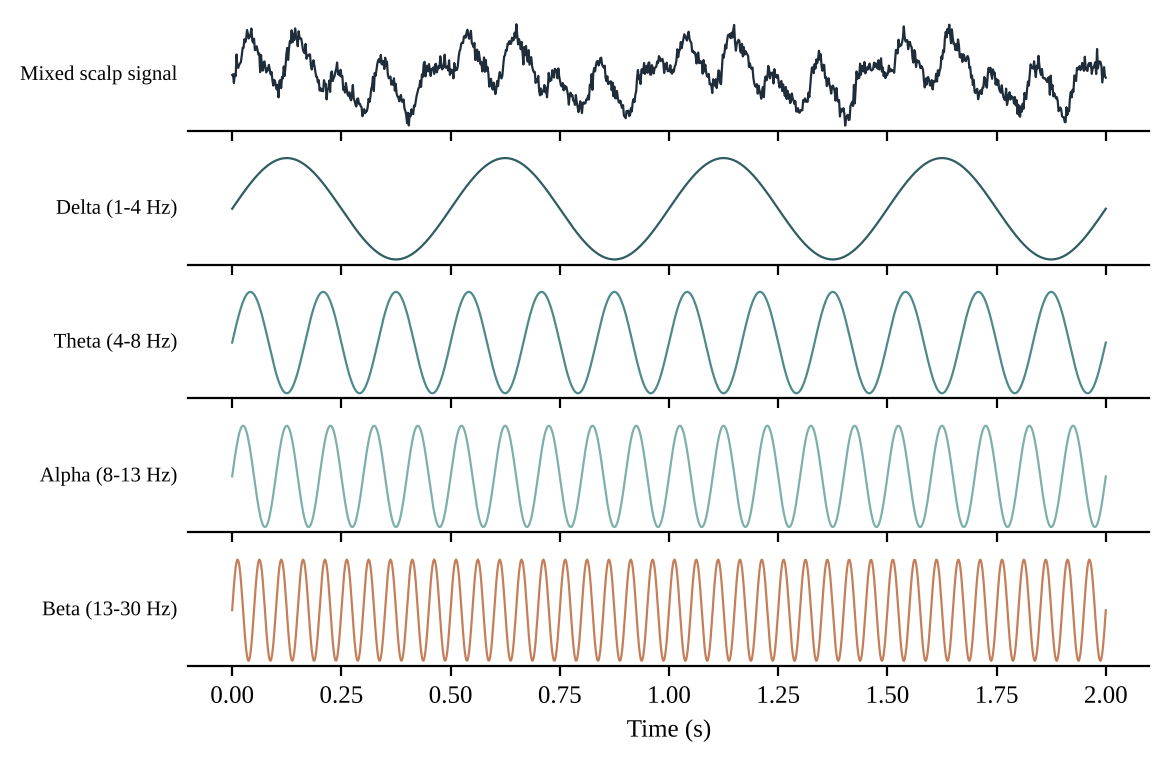
\includegraphics[width=0.85\textwidth]{fig_rhythms.png}
\caption[Illustration of a mixed EEG signal and four of the rhythms into which it is separated]{Illustration of a mixed EEG signal and four of the rhythms into which it is separated. The traces are synthetic sinusoids drawn only to illustrate the idea.}\label{fig:fig_rhythms}
\end{figure}
\begin{table}[!htbp]\centering\small\setstretch{1.1}
\caption{EEG frequency bands analysed in this project}\label{tab:bands}
\begin{tabularx}{\textwidth}{llX}
\toprule
Band & Range (Hz) & Typical context reported in the literature\\
\midrule
Delta ($\delta$) & 1--4 & Prominent in deep sleep\\
Theta ($\theta$) & 4--8 & Drowsiness and some memory processes\\
Alpha ($\alpha$) & 8--13 & Relaxed wakefulness, strongest with eyes closed\\
Beta ($\beta$) & 13--30 & Alert, active states; also affected by muscle activity\\
Gamma ($\gamma$) & > 30 & Not used: close to the 40 Hz filter edge and contaminated by muscle\\
\bottomrule
\end{tabularx}
\end{table}
The contexts in the last column vary with age, vigilance, drugs and the recording set-up, so they are given only as orientation; the models in this work do not attach any meaning to them. Likewise, frontal alpha asymmetry (FAA), often proposed as a marker of depression, did not show a reliable diagnostic effect in a meta-analysis \cite{faa}; it is included here as a feature to be tested, not as an assumption.


\section{Objectives}
The overall objective is a leakage-safe, reproducible benchmark that quantifies the accuracy cost and the privacy benefit of federated and differentially private training for EEG-based MDD classification. Three research questions guide the work:

\begin{description}[leftmargin=3.2em,labelwidth=2.6em,itemsep=2pt]
\item[RQ1] How well can MDD be separated from healthy controls on TDBRAIN when evaluation is strictly by participant, and is a compact deep network better than spectral features?
\item[RQ2] How much accuracy is lost by federated training, by non-identical client data, and by participant-level differential privacy at $\varepsilon$ $\in$ \{1, 3, 8\}?
\item[RQ3] How much membership leakage does each regime show under a participant-level LiRA attack, and how well do the frozen models transfer to an independent data set?
\end{description}
The specific objectives that follow from these questions are:

\begin{enumerate}[leftmargin=1.6em,itemsep=2pt,topsep=2pt]
\item Build a participant index from TDBRAIN (first session only, blinded and unknown labels excluded) and define two tasks: MDD vs healthy (T1) and MDD vs other diagnosed patients (T2).
\item Freeze participant-level cross-validation splits and simulated client partitions in a hashed file.
\item Preprocess each recording independently onto the 19 channels shared with the external data set.
\item Implement a spectral logistic-regression baseline and EEGNet-8,2 with group normalisation.
\item Train both under centralised, local-only, federated (FedAvg) and federated + participant-level DP regimes.
\item Audit privacy with a participant-level LiRA membership-inference attack.
\item Test the frozen models once on Mumtaz and probe whether the two data sets are trivially separable.
\item Log every run, generate the report and a dashboard from the logs, and package the work for reproduction.
\end{enumerate}

\section{Scope and Significance}
The scope is a computational benchmark on existing, de-identified recordings. It does not collect new data, does not diagnose, and does not recommend treatment. The four clients in the federated experiments are random partitions of one archive, not real hospitals.

What makes the work useful is the set of checks built around each number. Every experiment reads the same frozen splits; shuffling the labels tests for leakage; the privacy budget is counted per person and then challenged by an attack; an age-only model reveals how much a demographic difference explains; and the independent data set is opened a single time. A headline accuracy is only meaningful once these checks have been passed.


\section{Report Layout}
The remainder of the report is arranged as follows. Prior studies on EEG-based depression detection, federated learning, differential privacy and membership inference are surveyed in Chapter 2. Chapter 3 sets out the design of the benchmark, and Chapter 4 the cohort, preprocessing, models, privacy mechanism and evaluation protocol. The software stack is covered in Chapter 5, the experimental findings in Chapter 6, and the conclusions, limitations and next steps in Chapter 7.


\chapter{Related Work}

\section{EEG-Based Classification of Depression}
Spectral band power, inter-hemispheric asymmetry, connectivity and non-linear measures have all been studied as features for detecting depression from EEG \cite{review}. Mumtaz et al. recorded 34 patients with MDD and 30 healthy controls and reported accuracies close to 98\% with band power and alpha asymmetry \cite{mumtaz17}; that data set is public \cite{mumtazdata} and is used in this project only as an external test. Such results come from small single-centre samples, and the strongest reported effects have not replicated across data sets. In particular, a meta-analysis of frontal alpha asymmetry found no reliable diagnostic effect \cite{faa}.

TDBRAIN is a large clinical archive released by Brainclinics: 1,274 participants recorded between 2001 and 2021, including 426 with MDD and other groups such as ADHD, OCD and subjective memory complaints, with two minutes each of eyes-open and eyes-closed resting EEG on 26 channels \cite{tdbrain}. Its size and mixed clinical population make it a more realistic test bed than single-study samples.


\section{Data Leakage in EEG Studies}
Brookshire et al. reviewed deep-learning EEG studies and showed that splitting data by segment instead of by subject inflates accuracy, often dramatically, because a network learns person-specific signatures \cite{leak}. Small samples add a second problem: cross-validated estimates from a few hundred participants carry wide error bars \cite{varo}. This project therefore splits strictly by participant, reports participant-level bootstrap confidence intervals, and runs a shuffled-label control.


\section{Federated Learning}
In federated averaging (FedAvg), a server sends the current model to clients, each client trains on its own data, and the server averages the returned weights in proportion to client size \cite{fedavg}. When client data are not identically distributed, FedAvg can drift; FedProx adds a proximal term that keeps local models near the global one \cite{fedprox}, and FedBN keeps normalisation layers local \cite{fedbn}. Federated learning has been proposed as a route to multi-institution medical models \cite{rieke}, but keeping data on site does not by itself protect privacy: training data can be reconstructed from shared gradients \cite{dlg}.


\section{Differential Privacy}
A randomised mechanism is ($\varepsilon$, $\delta$)-differentially private if adding or removing one individual changes the probability of any output by at most a factor $e^{\varepsilon}$, except with probability $\delta$ \cite{dwork}. DP-SGD makes training private by clipping each example's gradient and adding Gaussian noise \cite{abadi}; the total privacy loss over many steps is tracked with Rényi differential privacy (RDP) \cite{rdp}, converted to ($\varepsilon$, $\delta$) with a tight bound \cite{balle}. McMahan et al. showed that the unit of privacy can be the \emph{user} rather than the example, by clipping and noising each user's whole contribution \cite{userdp}.

The unit matters for EEG. One person contributes many epochs, so a per-epoch guarantee --- what a standard per-sample accountant reports --- says little about the person. This project therefore uses participant-level DP and reports the epoch-level value only as a labelled comparison.


\section{Membership Inference}
A membership-inference attack asks whether a given record was in a model's training set \cite{shokri}. The likelihood-ratio attack (LiRA) of Carlini et al. trains shadow models with and without each target, fits Gaussians to the target's scores under both hypotheses, and reports the true-positive rate at low false-positive rates, which is more informative than average accuracy \cite{lira}. Here the attack is run at the participant level, so it measures exactly the risk that participant-level DP is meant to bound.


\section{Summary of Prior Work and the Gap}
\begin{table}[!htbp]\centering\small\setstretch{1.1}
\caption{How this work differs from the most relevant prior studies}\label{tab:related}
\begin{tabularx}{\textwidth}{llX}
\toprule
Work & Data & Relevance to this project\\
\midrule
Mumtaz et al. \cite{mumtaz17} & 64 people, 1 site & High accuracy from spectral features; used here as the external test\\
Brookshire et al. \cite{leak} & Review of EEG DL & Segment splits inflate accuracy; motivates subject-level splits and E12\\
van der Vinne et al. \cite{faa} & Meta-analysis & FAA is not a reliable marker; tested here as E16\\
McMahan et al. \cite{fedavg}, \cite{userdp} & Benchmarks & FedAvg and user-level DP; adapted to EEG participants\\
Carlini et al. \cite{lira} & Benchmarks & LiRA; adapted to participant-level membership\\
This project & TDBRAIN + Mumtaz & Leakage-safe benchmark of FL and participant-level DP with an attack audit and an external test\\
\bottomrule
\end{tabularx}
\end{table}
The gap is practical rather than conceptual. Each ingredient exists, but the combination --- subject-level splits, privacy accounted per participant, an attack that tests the guarantee, and an external data set --- has not been applied to EEG-based depression classification on a large clinical archive (Figure~\ref{fig:fig_gap}).

\begin{figure}[!htbp]\centering
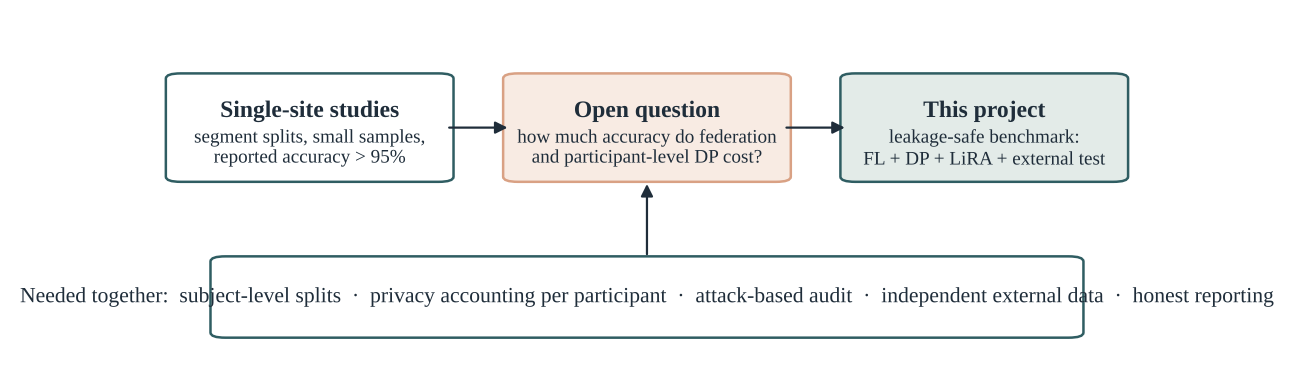
\includegraphics[width=0.95\textwidth]{fig_gap.png}
\caption[Where this project sits between existing single-site studies and the open question]{Where this project sits between existing single-site studies and the open question}\label{fig:fig_gap}
\end{figure}
\begin{table}[!htbp]\centering\small\setstretch{1.1}
\caption{Methodological risks and the safeguard adopted for each}\label{tab:difficulties}
\begin{tabularx}{\textwidth}{lX}
\toprule
Risk & Safeguard\\
\midrule
Segment-level leakage & Splits by participant, frozen and hashed; shuffled-label control (E01)\\
Optimistic small-sample estimates & Participant-level bootstrap CIs and paired differences\\
Per-epoch privacy says little about people & Participant-level DP; epoch-level $\varepsilon$ only as comparison\\
A guarantee without evidence & Participant-level LiRA attack (E10)\\
Results that only hold at one site & One-time external test on Mumtaz (E11) and a data-set probe (E13)\\
Demographic confounds & Age-only baseline (E22)\\
\bottomrule
\end{tabularx}
\end{table}

\chapter{Proposed System}

\section{System Overview}
The software is split into six layers with one responsibility each (Figure~\ref{fig:fig_architecture}). The \emph{data layer} builds the participant index and the frozen splits. The \emph{preprocessing layer} turns each recording into clean 4-second epochs on 19 channels. The \emph{model layer} holds the two tracks. The \emph{regime layer} trains them centrally, locally, federated or federated with DP. The \emph{evaluation layer} scores them per participant, attacks them and runs the external test. Tracking and reporting connect everything through MLflow.

\begin{figure}[!htbp]\centering
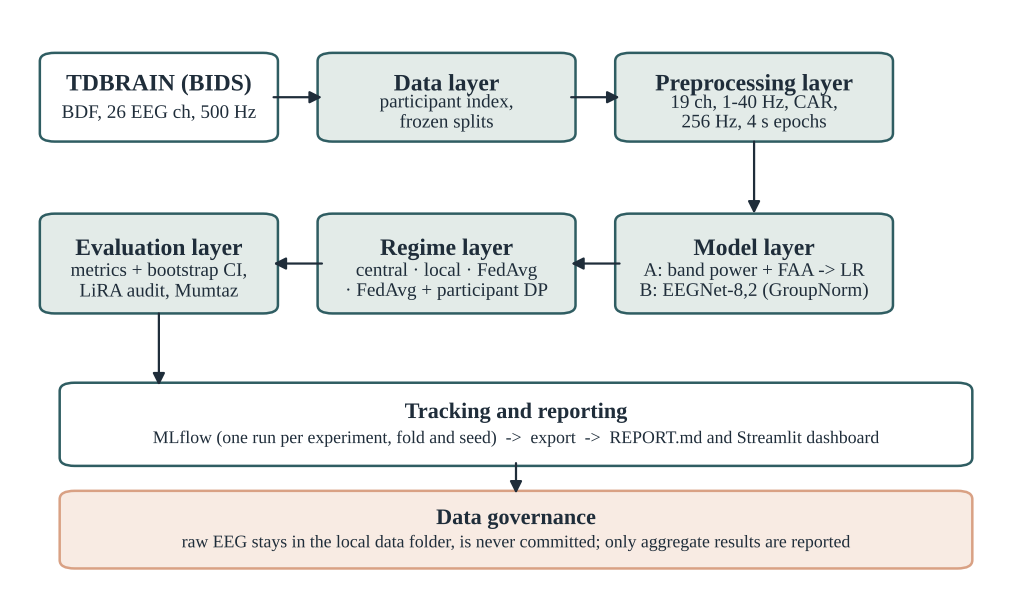
\includegraphics[width=0.95\textwidth]{fig_architecture.png}
\caption[Six-layer organisation of the benchmark software]{Six-layer organisation of the benchmark software}\label{fig:fig_architecture}
\end{figure}

\section{Design Principles}
\begin{itemize}[leftmargin=1.6em,itemsep=2pt,topsep=2pt]
\item \textbf{One split, made once.} Participants are split once and the file is hashed; every experiment reads it.
\item \textbf{Nothing is fitted on test data.} Scalers, thresholds, hyperparameters and early stopping use training or inner-validation participants only.
\item \textbf{The privacy unit is the participant.} Sampling, clipping and accounting all operate on people.
\item \textbf{The external set is touched once.} Only one module may read Mumtaz, and it logs every access.
\item \textbf{Every number comes from a logged run.} Reports and the dashboard are generated, never typed.
\item \textbf{Data never leave the local folder.} Raw EEG is never committed, uploaded or shown.
\end{itemize}

\section{System Requirements}
\begin{table}[!htbp]\centering\small\setstretch{1.1}
\caption{Functional requirements of the benchmark}\label{tab:fr}
\begin{tabularx}{\textwidth}{llX}
\toprule
ID & The system shall & How it is met\\
\midrule
FR1 & build a first-session participant index with task labels & src/data/index.py\\
FR2 & freeze participant-level splits and client partitions & splits.json with SHA-256 hash\\
FR3 & preprocess each recording without cross-subject statistics & src/preprocess/pipeline.py\\
FR4 & train two model tracks under four regimes & src/train, src/fl\\
FR5 & account privacy per participant & src/privacy/participant\_dp.py, accountant.py\\
FR6 & audit membership leakage & src/privacy/lira.py\\
FR7 & test frozen models once on an external set & src/eval/external.py\\
FR8 & log runs and generate the report and dashboard & MLflow, src/report, dashboard/\\
\bottomrule
\end{tabularx}
\end{table}
\begin{table}[!htbp]\centering\small\setstretch{1.1}
\caption{Quality attributes required of the benchmark}\label{tab:nfr}
\begin{tabularx}{\textwidth}{lX}
\toprule
Quality & Requirement\\
\midrule
Data governance & Raw EEG stays local; data folders are git-ignored; only aggregate results are reported\\
Leakage control & No participant in two sets or two clients; checked by automated tests\\
Reproducibility & Fixed seeds; config, split, data-table and git hashes stored with every run\\
Hardware & Runs on a CPU; uses CUDA or Apple MPS only if present\\
Honesty & Synthetic, budget-reduced and preliminary results are labelled wherever they appear\\
Safety of wording & No text claims diagnostic use or calls a feature a biomarker of depression\\
\bottomrule
\end{tabularx}
\end{table}

\section{Processing Pipeline}
Figure~\ref{fig:fig_pipeline} follows one recording through preprocessing. Each step operates on that recording alone, so no information passes between participants before the split is applied. A recording with too few clean epochs is excluded with its reason recorded; it is never silently dropped.

\begin{figure}[!htbp]\centering
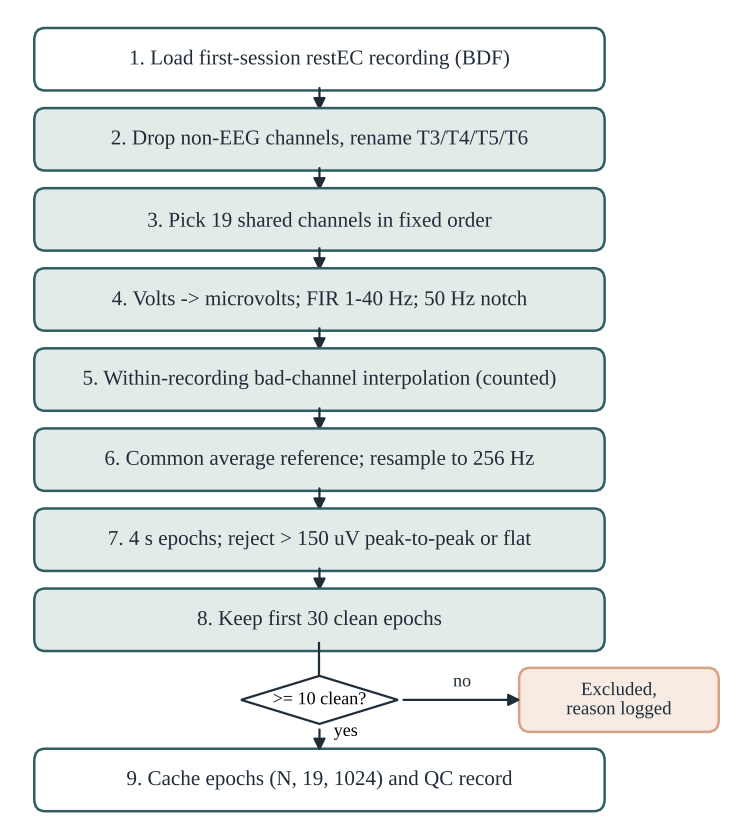
\includegraphics[width=0.62\textwidth]{fig_pipeline.png}
\caption[Preprocessing steps applied independently to every recording]{Preprocessing steps applied independently to every recording}\label{fig:fig_pipeline}
\end{figure}

\section{Training Regimes}
Each model recipe is trained in four ways (Figure~\ref{fig:fig_regimes}). In the \emph{centralised} regime all training participants are pooled, which gives an upper reference. In the \emph{local-only} regime each simulated client trains alone, which represents a single hospital. In the \emph{federated} regime the clients train locally and a server averages their weights. In the \emph{federated + DP} regime each client clips the contribution of every participant and adds Gaussian noise before its update leaves the client.

\begin{figure}[!htbp]\centering
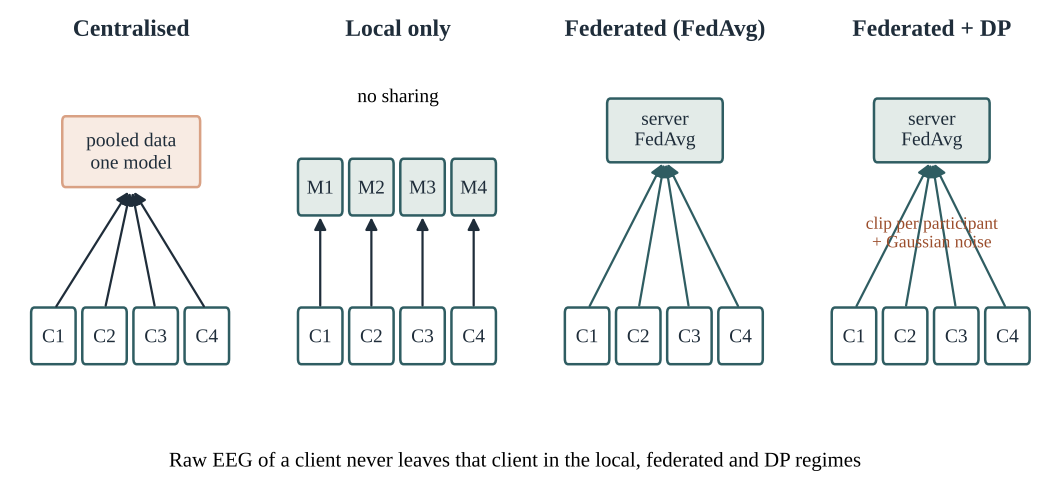
\includegraphics[width=0.98\textwidth]{fig_regimes.png}
\caption[The four training regimes]{The four training regimes. C1--C4 are the simulated clients}\label{fig:fig_regimes}
\end{figure}

\section{Current Completion State}
\begin{table}[!htbp]\centering\small\setstretch{1.1}
\caption{Completion state of each system component}\label{tab:status}
\begin{tabularx}{\textwidth}{lX}
\toprule
Component & Status\\
\midrule
Participant index, splits, preprocessing & Implemented and run on the full TDBRAIN release\\
Spectral LR, all four regimes & Implemented; all essential experiments run (5 folds)\\
EEGNet-8,2 & Implemented; run on fold 0 only under a reduced compute budget (preliminary)\\
Participant-level DP and accounting & Implemented, unit-tested and run for LR at $\varepsilon$ $\in$ \{1, 3, 8\}\\
LiRA audit & Run for LR, centralised and federated, at every $\varepsilon$\\
External test and data-set probe & Run once for LR models\\
Report, dashboard, tests, packaging & Implemented; 42 automated tests pass\\
Segment-split demonstration (E12), FedProx/FedBN, optional ablations & Implemented; not yet run on real data\\
\bottomrule
\end{tabularx}
\end{table}

\chapter{Material and Methodologies}

\section{Material}
Two data sets were used (Table~\ref{tab:data}). \textbf{TDBRAIN} (release V3) was obtained under its data-use agreement and contains BioSemi BDF recordings in a BIDS layout with 26 EEG channels plus eye, muscle and status channels at 500 Hz, and a participant table with 1363 session rows. \textbf{Mumtaz} is a public data set of 34 patients with MDD and 30 healthy controls recorded on 19 channels at 256 Hz with a linked-ear reference \cite{mumtazdata}.

\begin{table}[!htbp]\centering\small\setstretch{1.1}
\caption{Data used in this project}\label{tab:data}
\begin{tabularx}{\textwidth}{lXX}
\toprule
Property & TDBRAIN (training and cross-validation) & Mumtaz (external test only)\\
\midrule
Participants & 1303 (first session) & 34 MDD, 30 healthy\\
Channels & 26 EEG (+ 7 non-EEG) & 19 EEG (+ 3 non-EEG)\\
Sampling rate & 500 Hz & 256 Hz\\
Recording used & 2 min eyes closed (restEC) & Eyes closed (EC)\\
Labels & Clinical indication; replication sample blinded & MDD or healthy, from file names\\
Access & ORCID login and data-use agreement & Public (figshare)\\
\bottomrule
\end{tabularx}
\end{table}
The pipeline uses the 19 channels that both data sets share (Figure~\ref{fig:fig_montage}). In TDBRAIN's naming, Mumtaz's T3, T4, T5 and T6 are T7, T8, P7 and P8. Missing channels are never interpolated: using the intersection avoids inventing signal.

\begin{figure}[!htbp]\centering
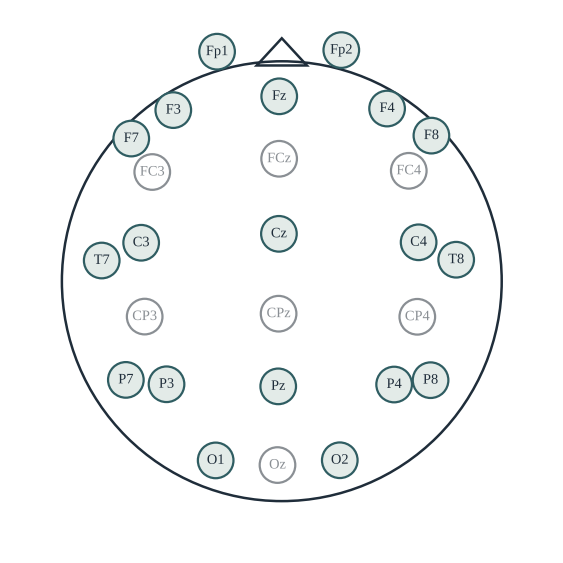
\includegraphics[width=0.50\textwidth]{fig_montage.png}
\caption[The 19 channels used (filled) and the TDBRAIN-only channels not used (grey), top view, nose upwards]{The 19 channels used (filled) and the TDBRAIN-only channels not used (grey), top view, nose upwards}\label{fig:fig_montage}
\end{figure}

\section{Cohort and Task Definitions}
Only each participant's first session was kept, because later sessions may follow treatment. Participants whose indication was missing or UNKNOWN (255) were excluded --- UNKNOWN does not mean healthy --- and the blinded replication sample is distributed separately. Adults aged 18--65 were kept. Two tasks were defined from the primary indication (Figure~\ref{fig:fig_cohort}): \textbf{T1}, MDD vs HEALTHY (n = 475), the primary task, and \textbf{T2}, MDD vs other diagnosed patients (n = 644).

\begin{figure}[!htbp]\centering
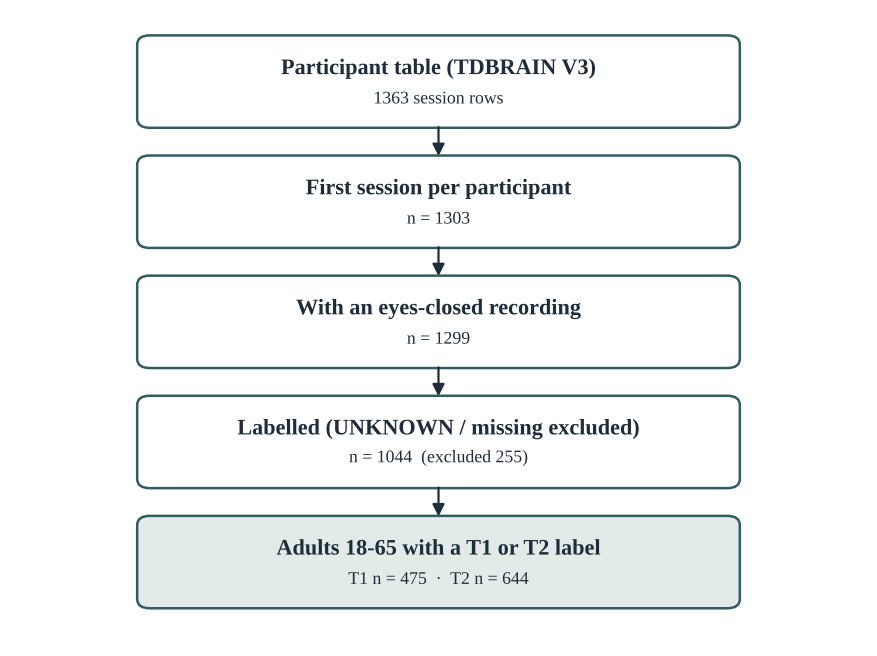
\includegraphics[width=0.70\textwidth]{fig_cohort.png}
\caption[Cohort flow from the participant table to the two tasks]{Cohort flow from the participant table to the two tasks}\label{fig:fig_cohort}
\end{figure}
\begin{table}[!htbp]\centering\small\setstretch{1.1}
\caption{Cohort per task and class (sex given as the raw code of the participant table)}\label{tab:cohort}
\begin{tabularx}{\textwidth}{llrrrr}
\toprule
Task & Class & n & Age, mean (SD) & Sex code 0 / 1 & Comorbid\\
\midrule
T1 & MDD & 313 & 43.4 (12.1) & 162 / 151 & 28\\
T1 & Healthy & 162 & 36.9 (14.1) & 93 / 69 & 0\\
T2 & Other patients & 331 & 43.8 (13.7) & 147 / 184 & 24\\
\bottomrule
\end{tabularx}
\end{table}
Healthy participants were on average 6.6 years younger than those with MDD. Because EEG power changes with age, an age-only baseline was added as a control (E22). The 'other patients' group of T2 is broad: the largest subgroups were ADHD (110), SMC (50) and OCD (42).


\section{Participant-Level Splits}
Splits were made once with stratified group 5-fold cross-validation, grouped by participant and stratified by label and age tertile (Figure~\ref{fig:fig_splits}). Inside each outer training fold, 20\% of the participants form an inner validation set used for hyperparameters, decision thresholds and early stopping. The remaining training participants are assigned to K = 4 clients, either at random (IID) or with label skew drawn from a Dirichlet distribution ($\alpha$ = 0.5) with at least five participants per class per client. The whole structure is saved to one file with a SHA-256 hash.

\begin{figure}[!htbp]\centering
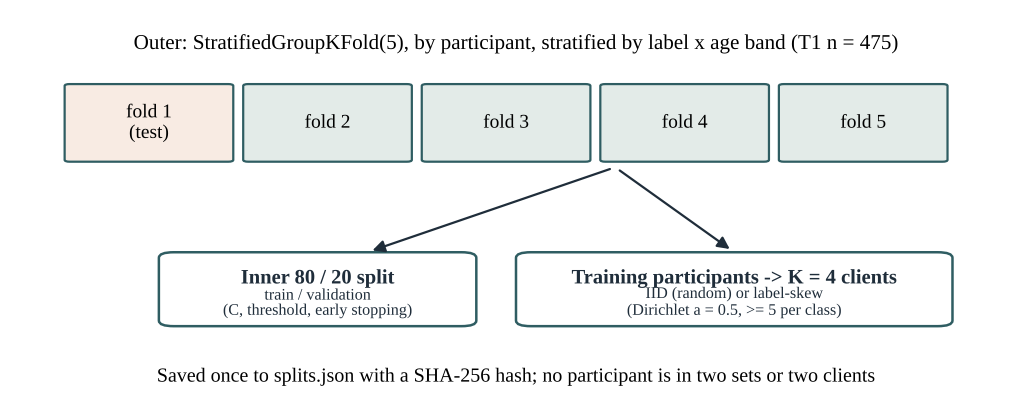
\includegraphics[width=0.95\textwidth]{fig_splits.png}
\caption[Participant-level splitting scheme]{Participant-level splitting scheme}\label{fig:fig_splits}
\end{figure}

\section{Preprocessing}
\begin{table}[!htbp]\centering\small\setstretch{1.1}
\caption{Preprocessing steps and settings}\label{tab:prep}
\begin{tabularx}{\textwidth}{lX}
\toprule
Step & Setting\\
\midrule
Channels & Non-EEG channels dropped; T3/T4/T5/T6 renamed; 19 channels picked in a fixed order\\
Units & Converted from volts to microvolts\\
Filtering & Zero-phase FIR band-pass 1--40 Hz; 50 Hz notch\\
Bad channels & Flat or outlying channels rebuilt by spherical-spline interpolation within the recording (at most 3; count logged)\\
Reference & Common average over the 19 channels\\
Resampling & 256 Hz\\
Epochs & 4 s (1,024 samples), non-overlapping\\
Rejection & Peak-to-peak above 150 \textmu{}V or below 1 \textmu{}V on any channel\\
Inclusion & At least 10 clean epochs; the first 30 clean epochs kept\\
\bottomrule
\end{tabularx}
\end{table}
Of 806 recordings with a task label, 10 (1.2\%) were excluded for too few clean epochs, 8.2\% of epochs were rejected, and 37 channels were interpolated in 28 recordings. As a sanity check, eyes-closed alpha power at O1/O2 exceeded that at Fp1/Fp2 in 95\% of participants, as expected from the posterior alpha rhythm (Figure~\ref{fig:fig_psd}).

\begin{figure}[!htbp]\centering
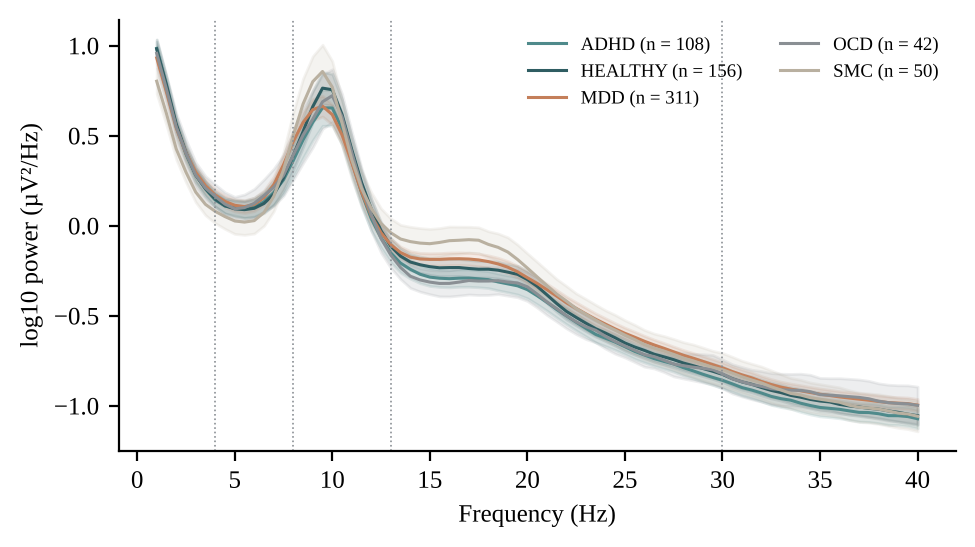
\includegraphics[width=0.80\textwidth]{fig_psd.png}
\caption[Group-mean eyes-closed power spectrum (19-channel mean, shaded 95\% interval of the mean) on TDBRAIN]{Group-mean eyes-closed power spectrum (19-channel mean, shaded 95\% interval of the mean) on TDBRAIN. Dotted lines mark the band edges}\label{fig:fig_psd}
\end{figure}

\section{Group-Level Description of the Signals}
Before any model is trained, it helps to look at how the two T1 groups differ on average. For each participant, the power in each band was divided by the total power between 1 and 30 Hz, giving relative power per channel; these maps were then averaged within each group (Figure~\ref{fig:fig_topo_bands}). Both groups show the expected posterior alpha maximum. On average the MDD group had lower occipital alpha (51.7\% vs 54.7\% at O1/O2), higher frontal-midline theta (19.5\% vs 17.2\% at Fz) and higher beta (19.6\% vs 17.2\% across channels). These are descriptive group means only: the groups also differ in age, and medication was not recorded, so the maps say nothing about cause.

\begin{figure}[!htbp]\centering
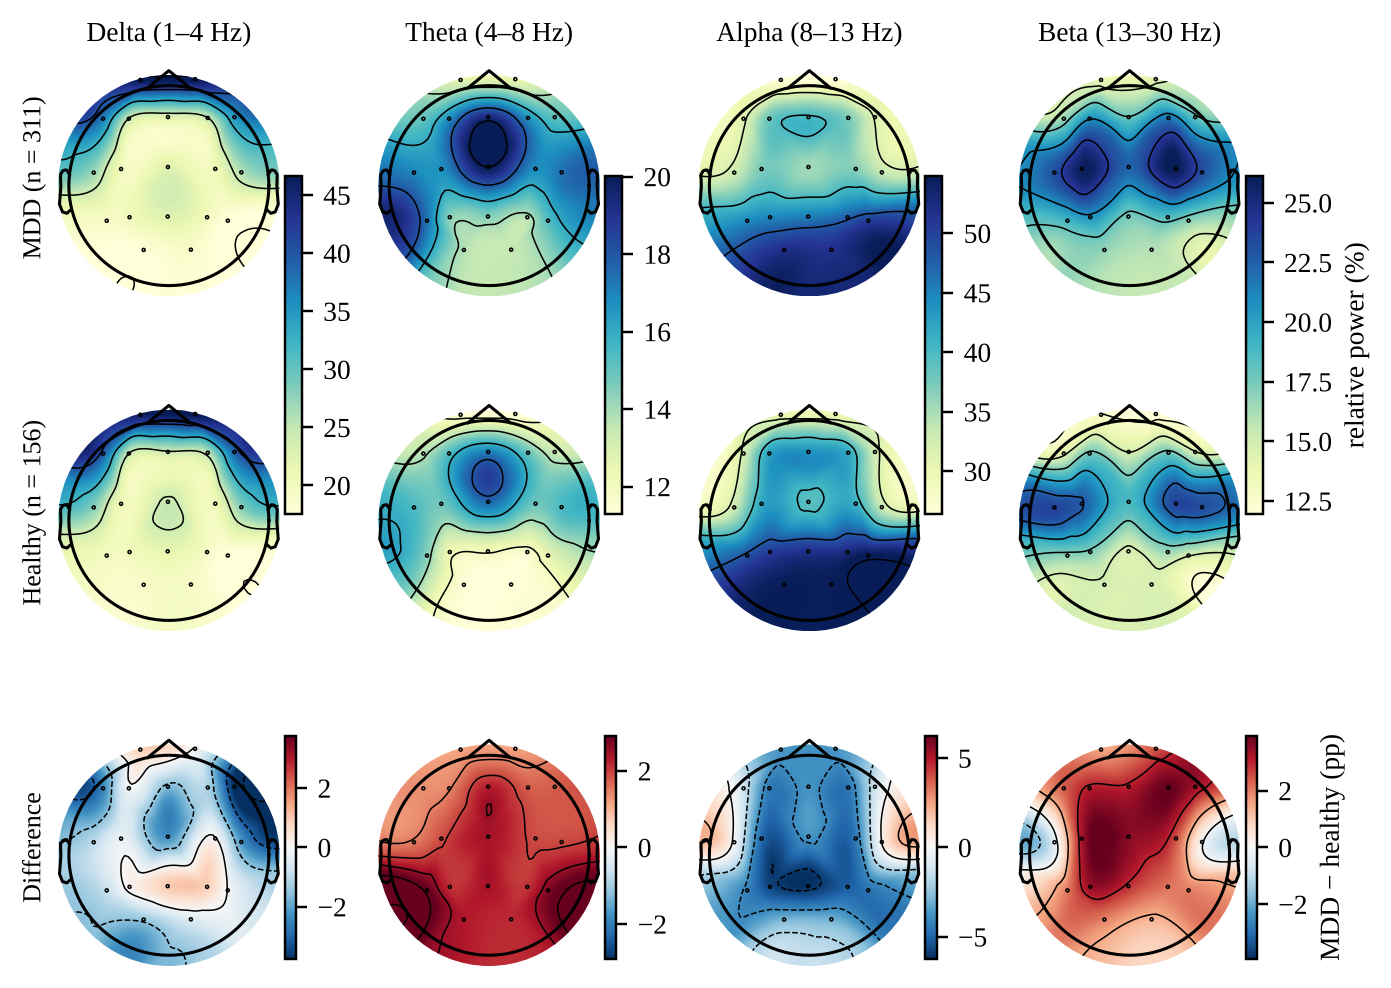
\includegraphics[width=0.98\textwidth]{fig_topo_bands.png}
\caption[Relative band power averaged over participants of each T1 group (top two rows; MDD n = 311, healthy n = 156) and the group difference in percentage points (bottom row)]{Relative band power averaged over participants of each T1 group (top two rows; MDD n = 311, healthy n = 156) and the group difference in percentage points (bottom row). Top view, nose upwards; dots mark the 19 electrodes}\label{fig:fig_topo_bands}
\end{figure}
Functional connectivity was summarised with the weighted phase-lag index (wPLI) in the alpha band, which ignores zero-lag coupling and is therefore less affected by volume conduction. Channel pairs were averaged within eleven scalp regions (Figure~\ref{fig:fig_conn_alpha}). Mean alpha wPLI was 0.291 in the MDD group and 0.275 in the healthy group; the differences are small compared with the spread within each matrix. Connectivity is not used as a model input in this project and is shown for description only.

\begin{figure}[!htbp]\centering
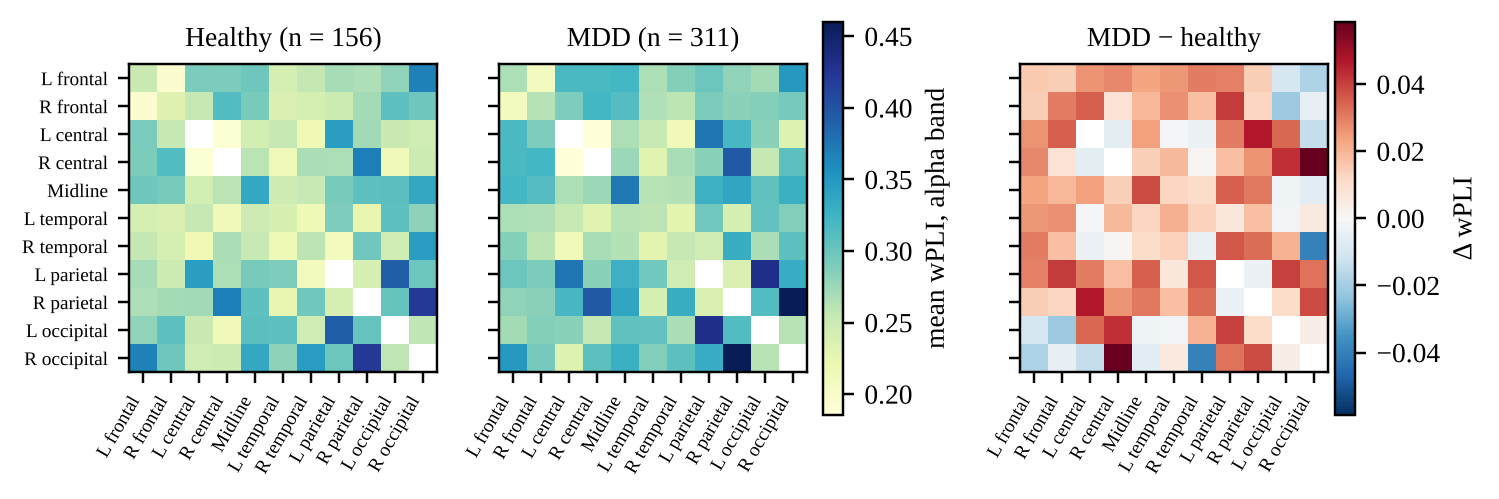
\includegraphics[width=0.98\textwidth]{fig_conn_alpha.png}
\caption[Alpha-band wPLI between scalp regions, averaged within each T1 group, and the difference between groups]{Alpha-band wPLI between scalp regions, averaged within each T1 group, and the difference between groups. Diagonal cells of single-channel regions are blank}\label{fig:fig_conn_alpha}
\end{figure}

\section{Spectral Features (Track A)}
For each epoch, Welch's method \cite{welch} with 2-second windows and 50\% overlap estimates the power spectrum of each channel. Absolute power is integrated over the delta, theta, alpha and beta bands and log-transformed, giving 19 $\times$ 4 = 76 features; frontal alpha asymmetry adds one more:

\begin{equation}
\mathrm{FAA} = \ln P_\alpha(\mathrm{F4}) - \ln P_\alpha(\mathrm{F3})
\end{equation}
Features are averaged over each participant's epochs. The centralised model is a standard scaler fitted on training participants, followed by L2-regularised logistic regression with balanced class weights \cite{sklearn}; the regularisation strength C $\in$ \{0.01, 0.1, 1, 10\} is chosen by inner-validation AUC and the decision threshold is then tuned on the same validation participants for balanced accuracy.


\section{EEGNet (Track B)}
Track B is EEGNet-8,2 \cite{eegnet} with group normalisation \cite{gn} in place of batch normalisation, because batch statistics mix participants and are awkward under federation and differential privacy (Figure~\ref{fig:fig_eegnet}). The network has 2,946 trainable parameters. Each recording is z-scored per channel using its own statistics only. Training uses Adam \cite{adam} (learning rate $10^{-3}$, batch 64) and class-weighted cross-entropy; early stopping monitors participant-level balanced accuracy on the inner validation set. A participant's probability is the mean of their epoch probabilities.

\begin{figure}[!htbp]\centering
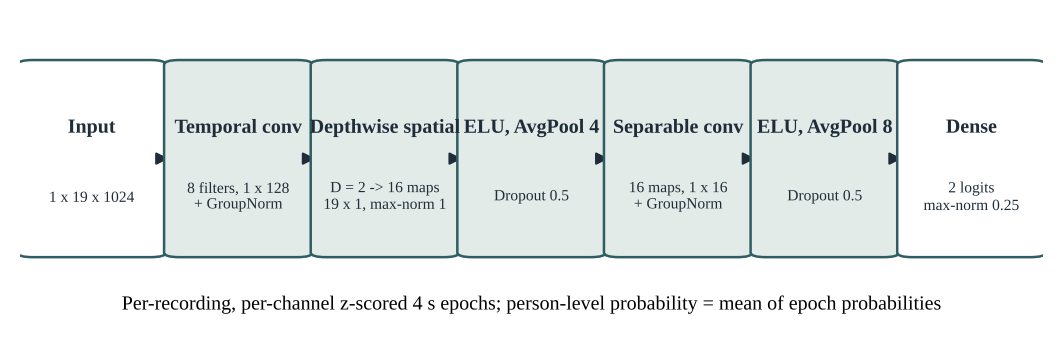
\includegraphics[width=0.98\textwidth]{fig_eegnet.png}
\caption[EEGNet-8,2 with group normalisation as used in this project]{EEGNet-8,2 with group normalisation as used in this project}\label{fig:fig_eegnet}
\end{figure}

\section{Federated Learning}
Federated training uses the Flower simulation engine \cite{flower} with one client per partition. Each round the server sends the global weights, every available client trains locally, and the server forms the weighted FedAvg \cite{fedavg}:

\begin{equation}
w_{t+1} = \sum_{k \in S_t} \frac{n_k}{\sum_{j \in S_t} n_j}\, w_{t+1}^{(k)}
\end{equation}
where n\_k is the size of client k and S\_t the clients available in round t. After every round the server evaluates the global model on the inner-validation participants and keeps the best round. For the linear model the feature scaler is computed from client sufficient statistics (sums and sums of squares), which equals the pooled training scaler without sharing raw features. A seeded dropout test makes each client unavailable with probability 0.2 per round. An equivalent in-process engine with the same client, selection and aggregation code was verified to produce identical weights and is used for speed.


\section{Participant-Level Differential Privacy}
Standard per-sample DP would treat each 4-second epoch as an individual. Here the participant is the unit (Figure~\ref{fig:fig_fl_dp}). At each local step a client samples each of its participants independently with probability q = 0.25, computes the gradient of each sampled participant's loss on one randomly chosen epoch, clips it to norm C = 1, and releases

\begin{equation}
\tilde g = \frac{1}{qN}\Big(\sum_{i \in B} g_i \min\big(1, \tfrac{C}{\lVert g_i \rVert_2}\big) + \mathcal{N}(0, \sigma^2 C^2 I)\Big)
\end{equation}
where N is the number of the client's participants. Per-participant gradients are obtained with vectorised automatic differentiation; the RDP accountant of Opacus \cite{opacus}, \cite{rdp} composes the steps of every round, and the reported $\varepsilon$ is the maximum over clients at $\delta$ = $10^{-5}$. For each target $\varepsilon$ the noise multiplier $\sigma$ is found by bisection; for logistic regression this gave $\sigma$ $\approx$ 3.31 ($\varepsilon$ = 8), 7.57 ($\varepsilon$ = 3) and 20.32 ($\varepsilon$ = 1). A pooled feature scaler would leak information outside the accounting, so DP logistic regression uses a per-participant transform instead (log band power relative to the participant's own channel mean, plus relative band levels), applied at every $\varepsilon$ including the non-private reference so that the comparison is like for like.

\begin{figure}[!htbp]\centering
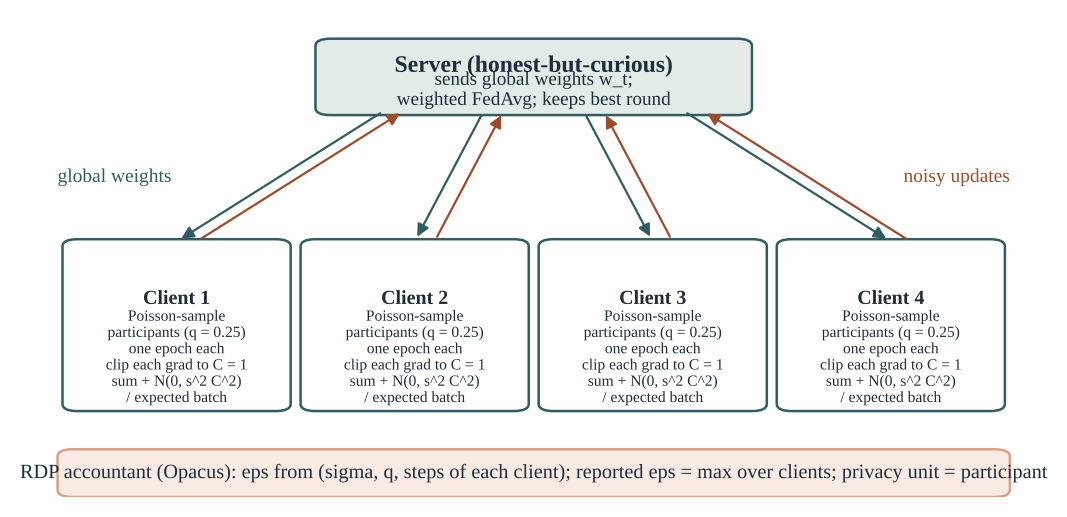
\includegraphics[width=0.95\textwidth]{fig_fl_dp.png}
\caption[One round of federated training with participant-level differential privacy]{One round of federated training with participant-level differential privacy}\label{fig:fig_fl_dp}
\end{figure}

\section{Privacy Audit (LiRA)}
The threat model is an honest-but-curious server, or anyone able to query the released model, who wants to know whether a given person's EEG was used in training. The audit follows LiRA \cite{lira} at the participant level (Figure~\ref{fig:fig_lira}). S models are trained with the target recipe, each on a random half of the labelled T1 pool; each participant's score is the mean, over their epochs, of the logit of the correct-class probability. Each model in turn is the target: for every participant the scores of the other models are split into members and non-members, Gaussians with a shared variance are fitted, and the likelihood ratio of the target's score is the attack statistic. The ROC, its AUC and the true-positive rates at 1\% and 5\% false-positive rate are reported; the rate at 0.1\% is reported only with at least 1,000 non-member evaluations.

\begin{figure}[!htbp]\centering
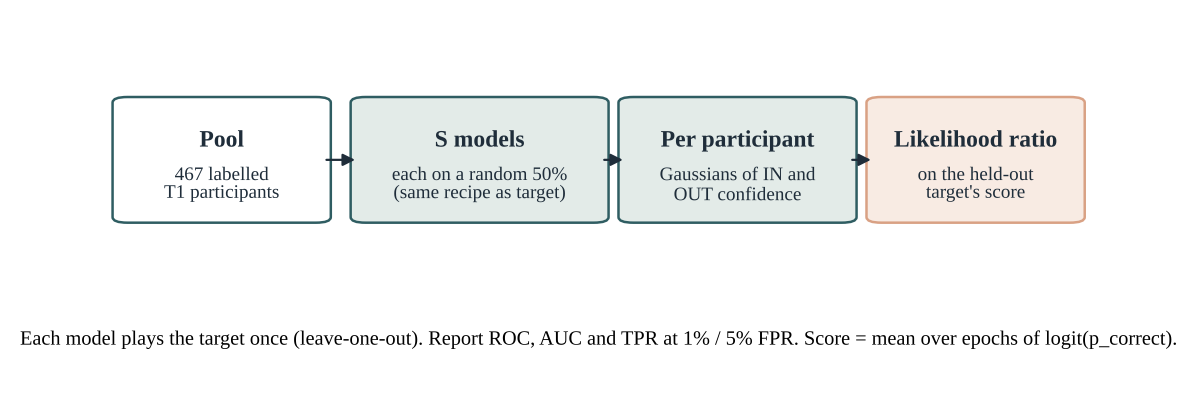
\includegraphics[width=0.95\textwidth]{fig_lira.png}
\caption[Participant-level likelihood-ratio membership-inference audit]{Participant-level likelihood-ratio membership-inference audit}\label{fig:fig_lira}
\end{figure}

\section{Evaluation and Statistics}
All metrics are computed per participant. Balanced accuracy and AUC are primary; sensitivity, specificity, F1, Matthews correlation and expected calibration error are also logged. Out-of-fold predictions are averaged over seeds per participant, and 95\% confidence intervals come from 2,000 class-stratified bootstrap resamples of participants \cite{boot}. Comparisons between configurations use a paired bootstrap of the difference on the same participants. No p-values from five-fold tests are reported as significant.


\section{External Test and Data-Set Probe}
For the external test, each model is retrained on all T1 participants with the hyperparameters chosen in cross-validation, and its decision threshold is fixed from TDBRAIN validation. Only then are the Mumtaz eyes-closed recordings loaded, preprocessed with the identical configuration, and scored once. A marker file prevents a second evaluation. The dataset-identity probe (E13) trains a logistic regression on band-power features to tell TDBRAIN healthy controls from Mumtaz healthy controls under grouped cross-validation; a high AUC means the two data sets differ in ways unrelated to diagnosis.

\begin{table}[!htbp]\centering\small\setstretch{1.1}
\caption{Experiment matrix (E22 was added during the project)}\label{tab:experiments}
\begin{tabularx}{\textwidth}{lXllX}
\toprule
ID & Question & Model & Regime & Status\\
\midrule
E01 & Shuffled-label control ($\approx$ 0.5) & LR, EEGNet & Centralised & Run (EEGNet fold 0)\\
E02 & Spectral baseline (T1) & LR & Centralised & Run\\
E03 & Harder contrast (T2) & LR & Centralised & Run\\
E04 & Deep vs features & EEGNet & Centralised & Run (fold 0)\\
E05 & Single-site loss & LR & Local only & Run\\
E06 & FL cost, IID vs label skew, dropout & LR & FedAvg & Run\\
E09 & Privacy cost, $\varepsilon$ $\in$ \{1, 3, 8, $\infty$\} & LR & FedAvg + DP & Run\\
E10 & LiRA audit & LR & Central, federated & Run\\
E11 & External transfer & LR & Frozen & Run once\\
E13 & Dataset-identity probe & LR & Centralised & Run\\
E16 & FAA alone & LR & Centralised & Run\\
E22 & Age alone (confound control) & LR & Centralised & Run\\
E07, E08, E12, E14--E21 & FedProx, FedBN, leakage demo, ablations & Both & Various & Implemented, not run\\
\bottomrule
\end{tabularx}
\end{table}

\chapter{Programming Language and Tools Used}

\section{Language and Core Libraries}
The system is written in Python 3.11 with a locked environment managed by uv. Table~\ref{tab:tools} lists the main libraries and their roles.

\begin{table}[!htbp]\centering\small\setstretch{1.1}
\caption{Libraries used, with version and purpose}\label{tab:tools}
\begin{tabularx}{\textwidth}{llX}
\toprule
Library & Version & Purpose in this project\\
\midrule
MNE-Python \cite{mne} & 1.13.2 & Reading BDF/EDF, filtering, referencing, interpolation\\
NumPy, SciPy, pandas & 2.2.6, 1.17.1, 3.1.1 & Arrays, Welch PSD, tables\\
scikit-learn \cite{sklearn} & 1.9.1 & Splits, logistic regression, metrics\\
PyTorch \cite{torch} & 2.15.0 & EEGNet, linear model, per-participant gradients\\
Flower \cite{flower} & 1.44.0 & Federated simulation (ClientApp / ServerApp)\\
Opacus \cite{opacus} & 1.6.0 & RDP privacy accountant\\
MLflow \cite{mlflow} & 3.18.0 & Run tracking, artefacts\\
Streamlit, Plotly & 1.67.0, 7.2.0 & Read-only results dashboard\\
pytest, ruff & --- & Automated tests and linting\\
\bottomrule
\end{tabularx}
\end{table}

\section{Code Organisation}
The code follows the layers of Figure~\ref{fig:fig_architecture}. Configuration lives in YAML files (data, preprocessing, models, federated learning, DP, audit) and in one file per experiment; an experiment runner expands each configuration into runs over variants, models, $\varepsilon$ values, folds and seeds. Named overlays (smoke, budget, fast, demo15) reduce the compute budget for quick passes and are recorded as a tag on every run.

\begin{table}[!htbp]\centering\small\setstretch{1.1}
\caption{Source packages and their responsibilities}\label{tab:modules}
\begin{tabularx}{\textwidth}{lX}
\toprule
Module & Responsibility\\
\midrule
src/data & Participant index, frozen splits, TDBRAIN and Mumtaz readers, downloads, synthetic test data\\
src/preprocess & Per-recording pipeline and QC report\\
src/features, src/models & Welch band power and FAA; logistic regression and EEGNet\\
src/train, src/fl & Centralised and local training; Flower client, server, strategy\\
src/privacy & Participant-level DP-SGD, RDP accountant, LiRA\\
src/eval & Metrics, bootstrap, external test (the only Mumtaz reader)\\
src/explain, src/report & Coefficients, spatial patterns, band occlusion; export, tables, figures\\
dashboard/ & Eight-page Streamlit application\\
\bottomrule
\end{tabularx}
\end{table}

\section{Data Governance and Privacy Measures}
\begin{itemize}[leftmargin=1.6em,itemsep=2pt,topsep=2pt]
\item TDBRAIN was obtained by the author under its data-use agreement; the copy used was the author's own private upload, checked to be private before download, and only the needed files were extracted.
\item Data folders, caches and EEG file types are excluded from version control, and the Docker image contains no data.
\item Credentials are stored outside the code and never printed or logged.
\item Only aggregate results appear in this report and the repository; per-participant predictions stay local.
\item A static test checks that no training module reads the external data set.
\end{itemize}

\section{Experiment Tracking and Reproducibility}
Every run is logged to MLflow with its configuration, configuration hash, split hash, participant-table hash, git commit, seed, metrics, confusion matrix, $\varepsilon$, checkpoint and per-participant predictions. An export step aggregates the runs into result tables, from which the report and the dashboard are generated. The results in Chapter 6 come from 157 logged runs.


\section{The Dashboard}
A read-only Streamlit dashboard presents the results in eight pages: overview, cohort and QC, model performance, federated learning, privacy, external test, explainability and reproducibility. It needs no credentials, accepts no uploads, and reads only the exported result files (Figure~\ref{fig:dash_privacy}).

\begin{figure}[!htbp]\centering
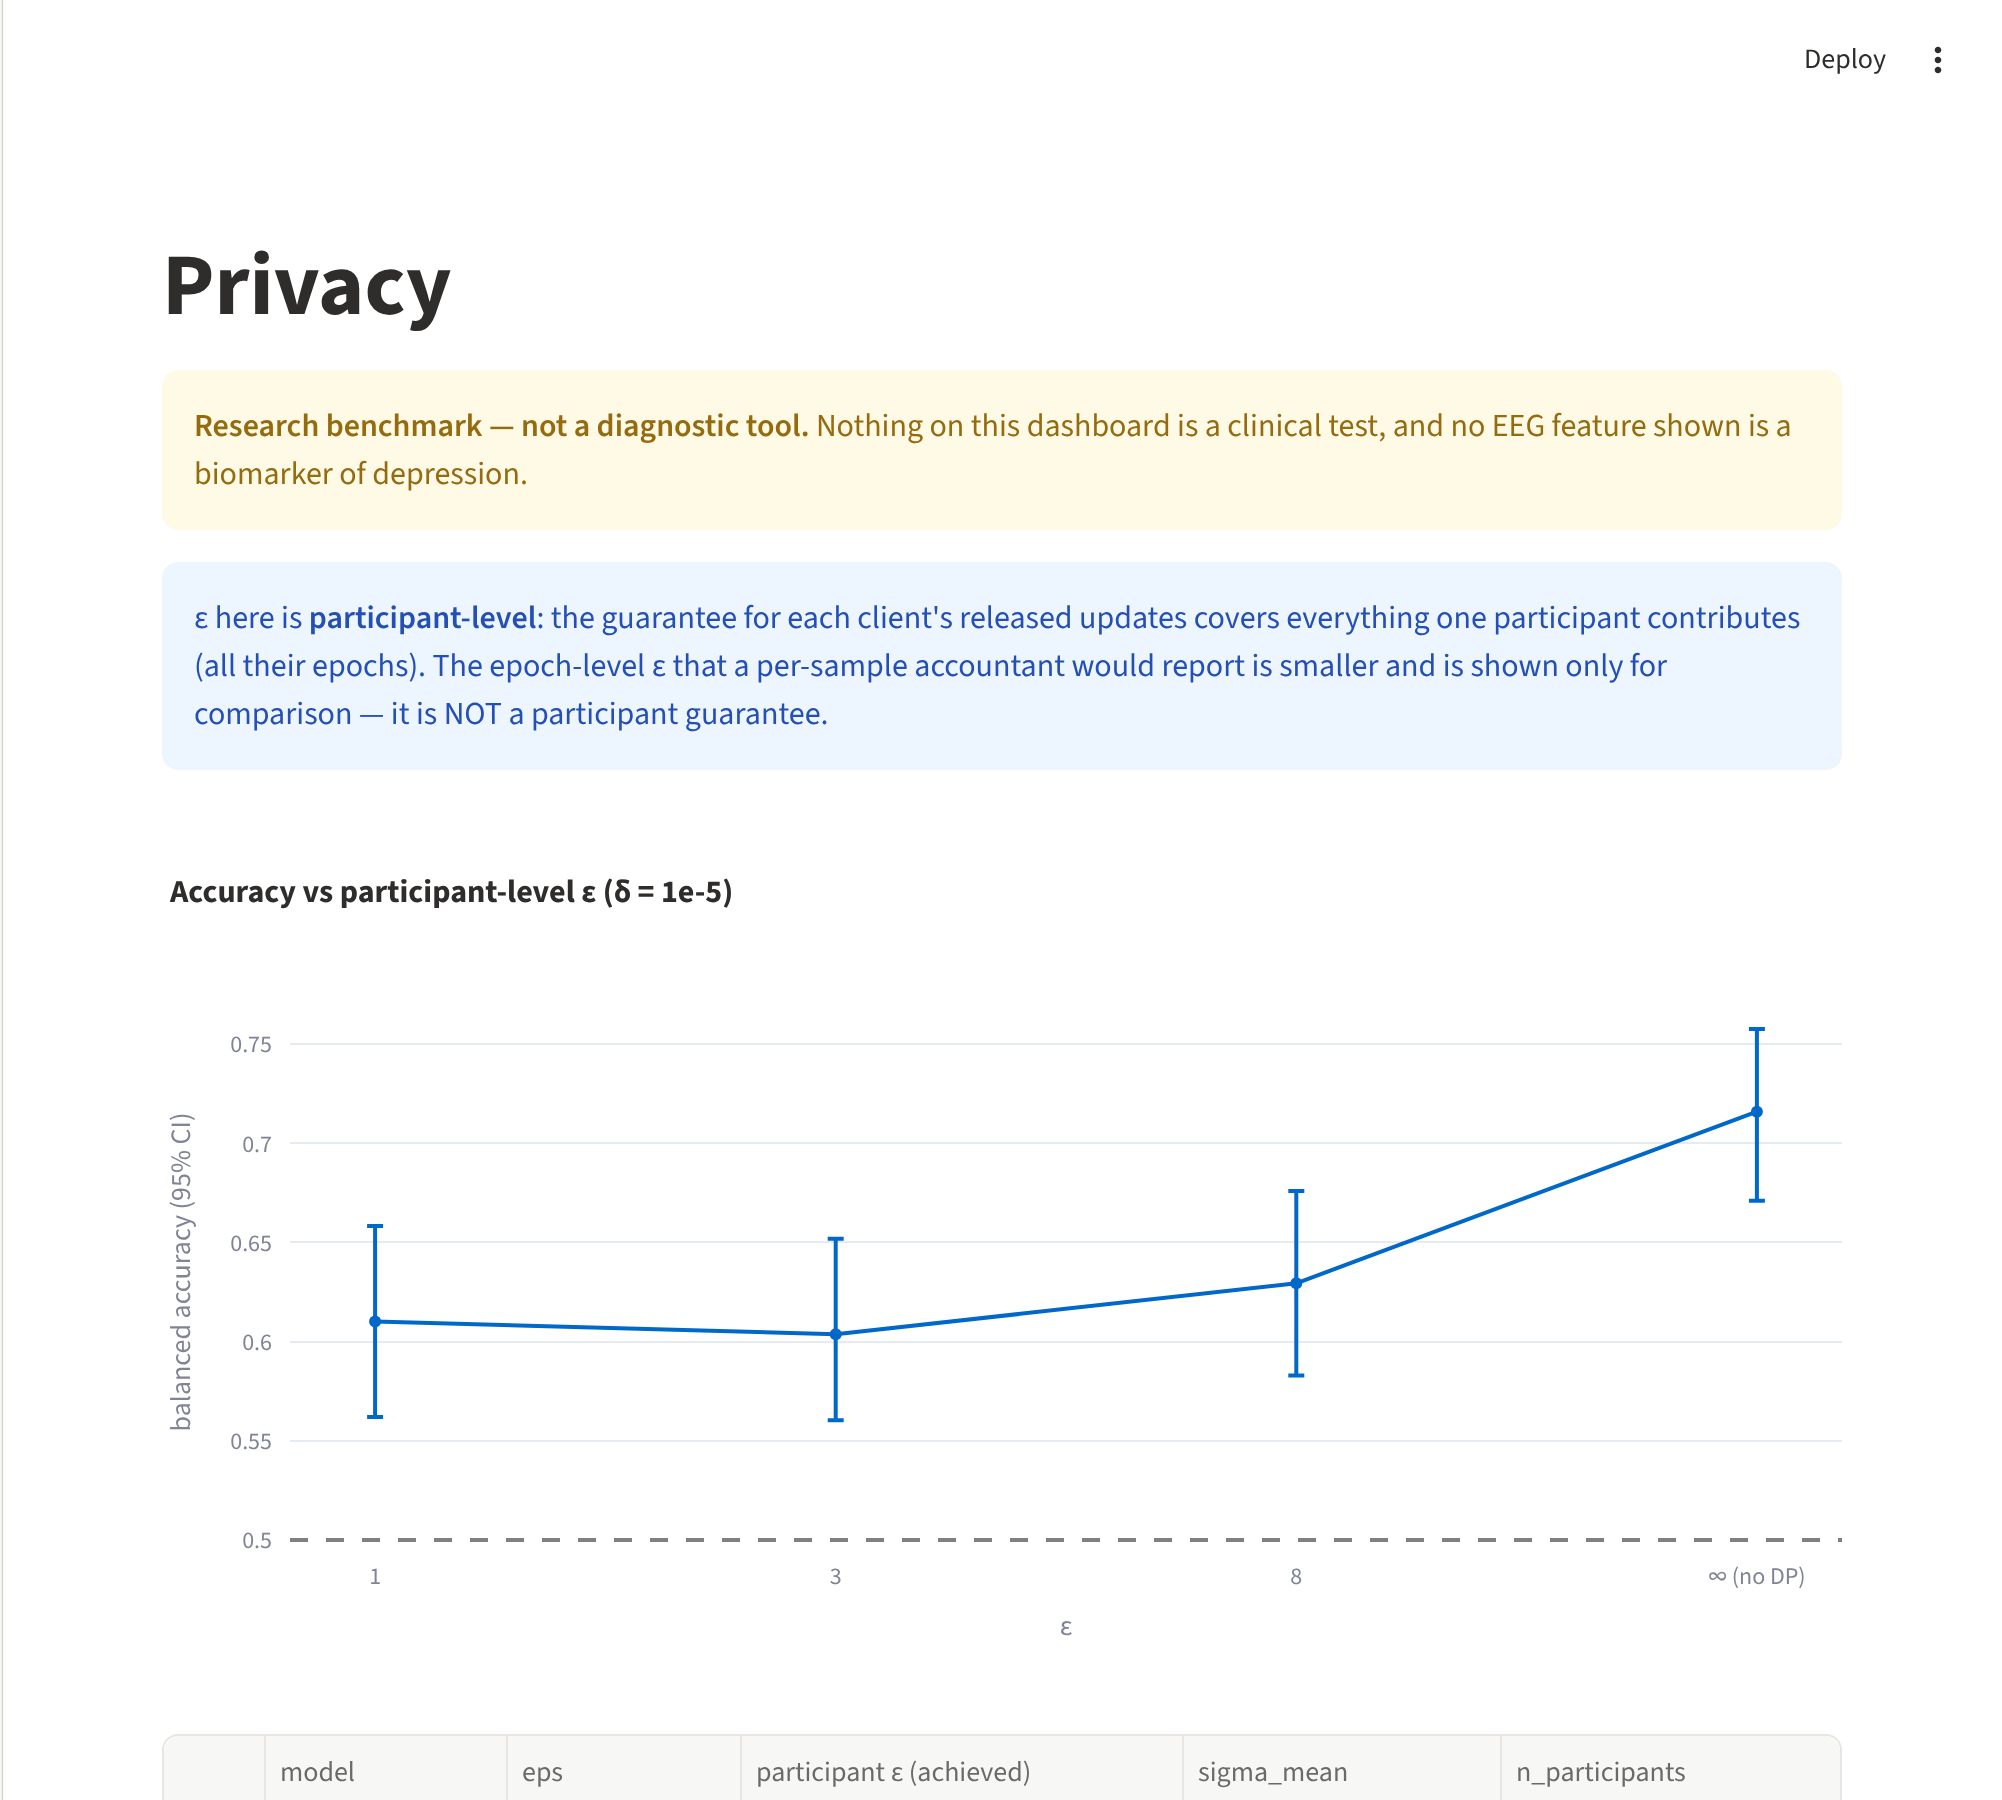
\includegraphics[width=0.80\textwidth]{dash_privacy.png}
\caption[The privacy page of the dashboard, generated from the logged TDBRAIN runs]{The privacy page of the dashboard, generated from the logged TDBRAIN runs}\label{fig:dash_privacy}
\end{figure}

\section{Testing}
\begin{table}[!htbp]\centering\small\setstretch{1.1}
\caption{Automated tests (42 in total, all passing)}\label{tab:tests}
\begin{tabularx}{\textwidth}{lX}
\toprule
Area & What is checked\\
\midrule
Splits & No participant in two sets or two clients; one test fold each; stable hash; tamper detection\\
Preprocessing & Shape (n, 19, 1024), channel order, microvolt scale, 256 Hz, no NaN, renaming, BDF files\\
No test fitting & Scaler, threshold and early stopping receive only training or validation participants\\
Differential privacy & Clipping bound per participant, noise scale, accountant against an analytic value\\
Federated learning & K = 1 federated equals centralised; Flower engine equals the in-process engine\\
LiRA & AUC > 0.9 when members are separable; $\approx$ 0.5 with no membership effect\\
Isolation and controls & Only the external module reads Mumtaz; the E01 check fails on a leaky positive control\\
\bottomrule
\end{tabularx}
\end{table}

\chapter{Results and Analysis}

\section{Experimental Setup}
All experiments ran on a 4-core CPU without a graphics card. Logistic-regression experiments used the full five folds; E01--E05, E16 and E22 used three seeds and E06, E09 and E10 one seed with 20 federated rounds and 16 LiRA models per configuration. EEGNet was run only on fold 0 with at most 15 passes (E01) or 8 passes (E04), because one model took several minutes on this hardware; its results are therefore preliminary. All figures and tables below are generated from the logged runs.


\section{Leakage Control}
With shuffled training labels the spectral model reached a balanced accuracy of 0.494 [0.446, 0.541] and an AUC of 0.457 on 467 participants, and EEGNet 0.539 on fold 0. Both are consistent with chance, so the pipeline does not leak label information into the test folds.


\section{Centralised Results}
\begin{table}[!htbp]\centering\small\setstretch{1.1}
\caption{Centralised results (participant level, 95\% bootstrap CI)}\label{tab:central}
\begin{tabularx}{\textwidth}{XrllXX}
\toprule
Configuration & n & Balanced accuracy & AUC & Sens. & Spec.\\
\midrule
E01 shuffled labels & 467 & 0.494 [0.446, 0.541] & 0.457 [0.402, 0.512] & 0.347 & 0.641\\
E02 band power + FAA & 467 & 0.738 [0.693, 0.780] & 0.768 [0.720, 0.814] & 0.759 & 0.718\\
E16 FAA only & 467 & 0.538 [0.491, 0.584] & 0.536 [0.477, 0.594] & 0.447 & 0.628\\
E22 age only & 467 & 0.615 [0.568, 0.663] & 0.635 [0.580, 0.693] & 0.704 & 0.526\\
E03 T2: MDD vs other patients & 640 & 0.553 [0.514, 0.590] & 0.581 [0.536, 0.624] & 0.383 & 0.723\\
E04 EEGNet (fold 0) & 94 & 0.663 [0.566, 0.760] & 0.724 [0.611, 0.823] & 0.810 & 0.516\\
\bottomrule
\end{tabularx}
\end{table}
The spectral baseline reached 0.738 [0.693, 0.780] balanced accuracy on T1 (Figure~\ref{fig:fig_main_results}). Two controls qualify this. First, age alone reached 0.615; the band-power model was better by 0.123 [0.067, 0.180], so it carries information beyond age, but part of its performance is likely age-related. Second, FAA alone was close to chance (0.538), 0.201 below the full model, which agrees with the meta-analysis \cite{faa}. The harder T2 contrast fell to 0.553, showing that the features separate depression from health much better than from other clinical groups.

\begin{figure}[!htbp]\centering
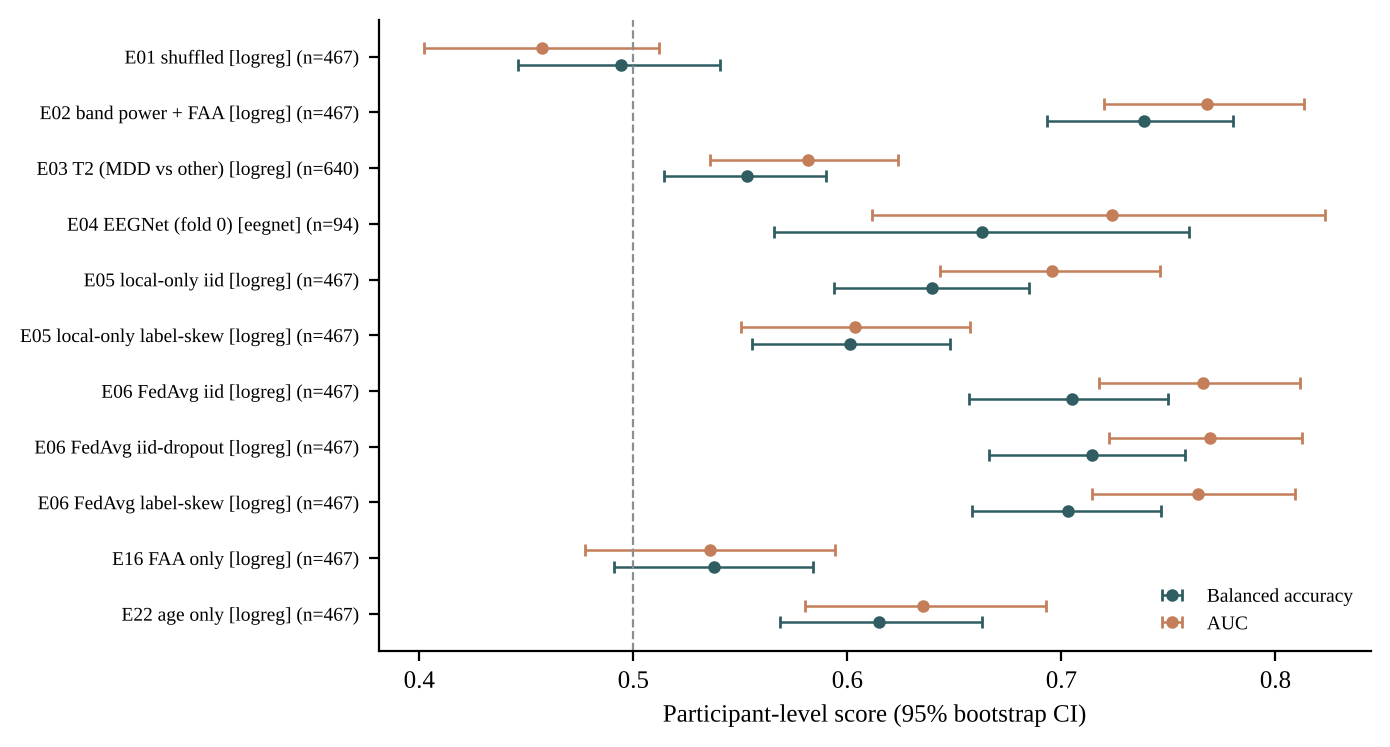
\includegraphics[width=0.98\textwidth]{fig_main_results.png}
\caption[Participant-level balanced accuracy and AUC with 95\% bootstrap intervals]{Participant-level balanced accuracy and AUC with 95\% bootstrap intervals}\label{fig:fig_main_results}
\end{figure}
On fold 0, EEGNet reached 0.663 balanced accuracy and AUC 0.724. Paired with the spectral model on the same 94 participants, the difference was -0.008 [-0.113, 0.096]: under this budget the deep model did not outperform the features, and the interval is too wide for a conclusion.

\begin{figure}[!htbp]\centering
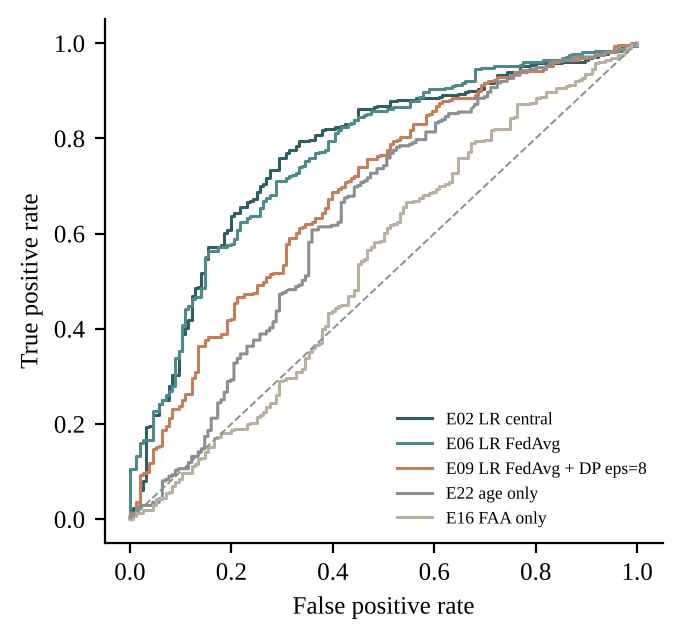
\includegraphics[width=0.55\textwidth]{fig_roc.png}
\caption[ROC curves of the logistic-regression configurations (seed-averaged out-of-fold predictions)]{ROC curves of the logistic-regression configurations (seed-averaged out-of-fold predictions)}\label{fig:fig_roc}
\end{figure}

\section{Federated and Local Training}
\begin{table}[!htbp]\centering\small\setstretch{1.1}
\caption{Federated and local-only logistic regression on T1}\label{tab:fl}
\begin{tabularx}{\textwidth}{Xllr}
\toprule
Regime & Balanced accuracy & AUC & Worst client BA\\
\midrule
Centralised & 0.738 [0.693, 0.780] & 0.768 [0.720, 0.814] & ---\\
FedAvg, IID & 0.705 [0.657, 0.750] & 0.766 [0.717, 0.811] & ---\\
FedAvg, label skew & 0.703 [0.658, 0.746] & 0.764 [0.714, 0.809] & ---\\
FedAvg, IID, 20\% client dropout & 0.714 [0.666, 0.758] & 0.769 [0.722, 0.812] & ---\\
Local only, IID (mean client) & 0.640 [0.594, 0.685] & 0.695 [0.643, 0.746] & 0.620\\
Local only, label skew (mean client) & 0.601 [0.555, 0.648] & 0.604 [0.550, 0.657] & 0.592\\
\bottomrule
\end{tabularx}
\end{table}
FedAvg lost 0.034 [0.005, 0.066] in balanced accuracy against centralised training, with no measurable loss in AUC (-0.002). Label skew changed the federated result by only -0.002, and random client dropout had no visible effect. Training on a single simulated site, in contrast, lowered balanced accuracy to 0.640 (IID) and 0.601 (label skew) (Figure~\ref{fig:fig_fl}). For a linear model on these features, federation therefore recovers most of what pooling would give, which is the practical case for it.

\begin{figure}[!htbp]\centering
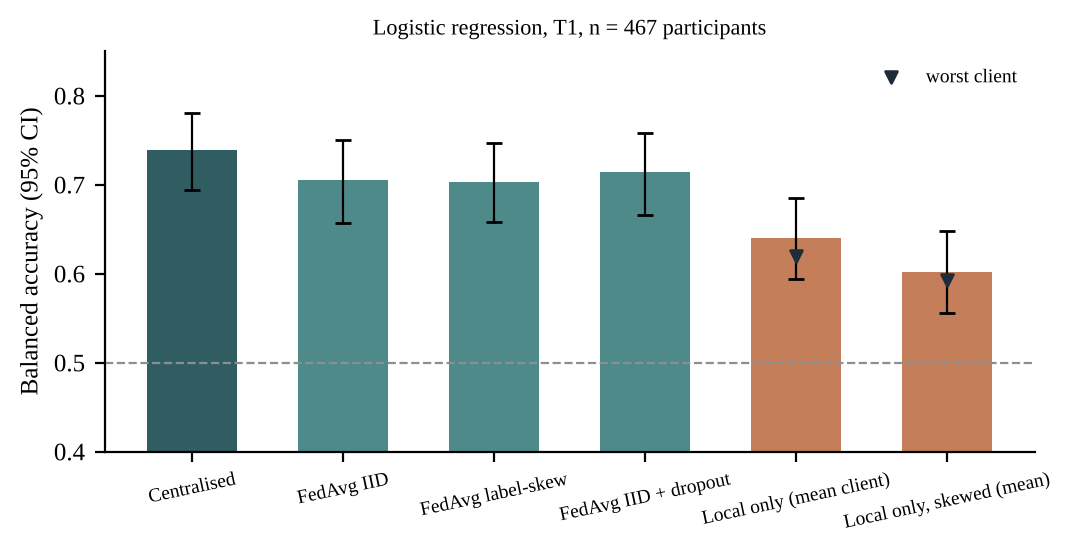
\includegraphics[width=0.90\textwidth]{fig_fl.png}
\caption[Centralised, federated and local-only logistic regression (worst client marked for local-only)]{Centralised, federated and local-only logistic regression (worst client marked for local-only)}\label{fig:fig_fl}
\end{figure}

\section{Cost of Participant-Level Privacy}
\begin{table}[!htbp]\centering\small\setstretch{1.1}
\caption{Federated logistic regression with participant-level DP ($\delta$ = $10^{-5}$)}\label{tab:dp}
\begin{tabularx}{\textwidth}{rrrXXX}
\toprule
Target $\varepsilon$ & Achieved $\varepsilon$ & $\sigma$ & Balanced accuracy & AUC & $\Delta$ BA vs $\varepsilon$ = $\infty$\\
\midrule
8 & 8.00 & 3.31 & 0.629 [0.583, 0.676] & 0.688 [0.637, 0.737] & -0.086 [-0.133, -0.040]\\
3 & 3.00 & 7.57 & 0.604 [0.560, 0.652] & 0.639 [0.583, 0.693] & -0.112 [-0.164, -0.058]\\
1 & 1.00 & 20.32 & 0.610 [0.562, 0.658] & 0.641 [0.584, 0.693] & -0.106 [-0.160, -0.051]\\
$\infty$ & --- & --- & 0.716 [0.671, 0.758] & 0.767 [0.718, 0.814] & ---\\
\bottomrule
\end{tabularx}
\end{table}
Participant-level DP cost between 0.086 ($\varepsilon$ = 8) and 0.112 ($\varepsilon$ = 3) in balanced accuracy relative to the non-private reference with the same features (Figure~\ref{fig:fig_privacy}). Accuracy remained clearly above chance even at $\varepsilon$ = 1. Because each participant contributes a single averaged feature vector to this model, an epoch-level $\varepsilon$ is not defined for it; for EEGNet it would be much smaller than the participant-level value and would overstate the protection.

\begin{figure}[!htbp]\centering
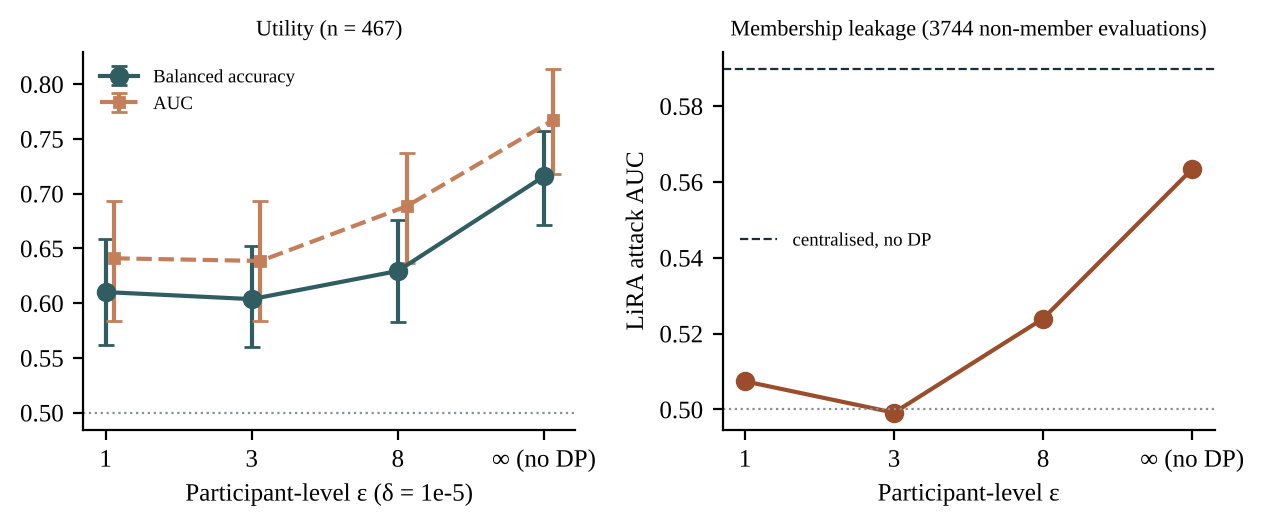
\includegraphics[width=0.98\textwidth]{fig_privacy.png}
\caption[Privacy--utility trade-off: accuracy (left) and LiRA attack AUC (right) against participant-level $\varepsilon$]{Privacy--utility trade-off: accuracy (left) and LiRA attack AUC (right) against participant-level $\varepsilon$}\label{fig:fig_privacy}
\end{figure}

\section{Privacy Audit}
\begin{table}[!htbp]\centering\small\setstretch{1.1}
\caption{Participant-level LiRA audit of logistic regression (0.5 = chance)}\label{tab:lira}
\begin{tabularx}{\textwidth}{llrrrr}
\toprule
Regime & $\varepsilon$ & Attack AUC & TPR @ 1\% FPR & TPR @ 5\% FPR & Sanity AUC\\
\midrule
Centralised & $\infty$ & 0.590 & 0.017 & 0.075 & 0.485\\
Federated & $\infty$ & 0.563 & 0.023 & 0.089 & 0.512\\
Federated & 8 & 0.524 & 0.014 & 0.064 & 0.489\\
Federated & 3 & 0.499 & 0.013 & 0.059 & 0.509\\
Federated & 1 & 0.507 & 0.014 & 0.054 & 0.498\\
\bottomrule
\end{tabularx}
\end{table}
Without DP the attack had a modest but real advantage: AUC 0.590 for the centralised model and 0.563 for the federated one. With participant-level DP the advantage almost disappeared (AUC 0.524 at $\varepsilon$ = 8 and 0.499--0.507 at $\varepsilon$ $\leq$ 3), and the true-positive rate at 1\% FPR fell to the level expected by chance (Figure~\ref{fig:fig_lira_roc}). The sanity check --- relabelling a random half of non-members as members --- gave AUC close to 0.5 everywhere. With 3744 non-member evaluations per configuration, the rate at 0.1\% FPR could also be estimated. Federation alone reduced leakage only slightly; the formal guarantee came from DP.

\begin{figure}[!htbp]\centering
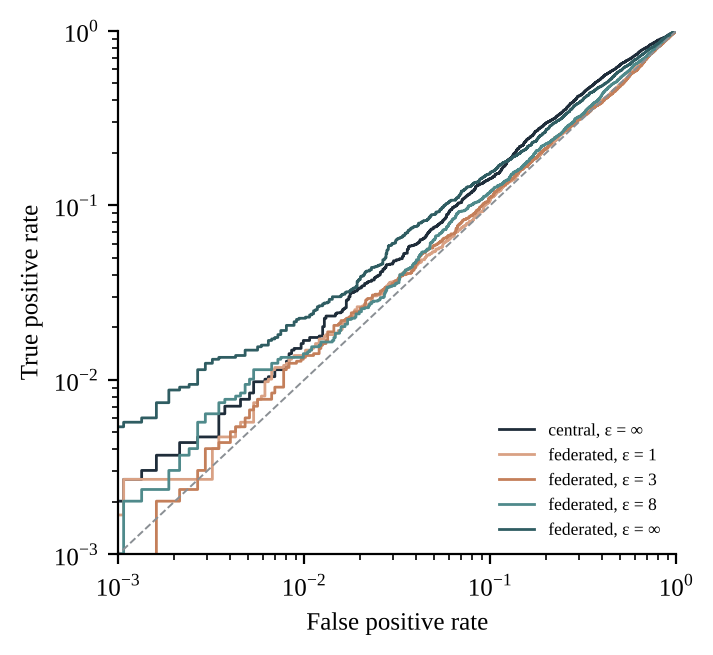
\includegraphics[width=0.55\textwidth]{fig_lira_roc.png}
\caption[LiRA ROC on log--log axes for logistic regression]{LiRA ROC on log--log axes for logistic regression}\label{fig:fig_lira_roc}
\end{figure}

\section{External Test and Data-Set Probe}
\begin{table}[!htbp]\centering\small\setstretch{1.1}
\caption{One-time external test on Mumtaz eyes-closed recordings (n = 58)}\label{tab:external}
\begin{tabularx}{\textwidth}{lllrr}
\toprule
Model & Balanced accuracy & AUC & Sensitivity & Specificity\\
\midrule
LR centralised & 0.679 [0.589, 0.768] & 0.549 [0.382, 0.707] & 1.000 & 0.357\\
LR FedAvg & 0.645 [0.542, 0.751] & 0.536 [0.365, 0.696] & 0.933 & 0.357\\
LR FedAvg + DP, $\varepsilon$ = 8 & 0.593 [0.489, 0.698] & 0.660 [0.517, 0.789] & 0.900 & 0.286\\
\bottomrule
\end{tabularx}
\end{table}
Transfer to Mumtaz was weak (Figure~\ref{fig:fig_external}). The AUCs (0.549--0.660) were close to chance with wide intervals, and the fixed TDBRAIN thresholds labelled almost every Mumtaz participant as MDD (sensitivity 1.000, specificity 0.357), so the balanced accuracies should not be read as successful transfer. The data-set probe explains why: band power separated TDBRAIN and Mumtaz healthy controls with AUC 0.966 [0.935, 0.990]. Amplifier, reference, country and population differ so much that a model trained on one archive meets a shifted feature distribution on the other. This is the main reason the design keeps Mumtaz strictly external rather than pooling it.

\begin{figure}[!htbp]\centering
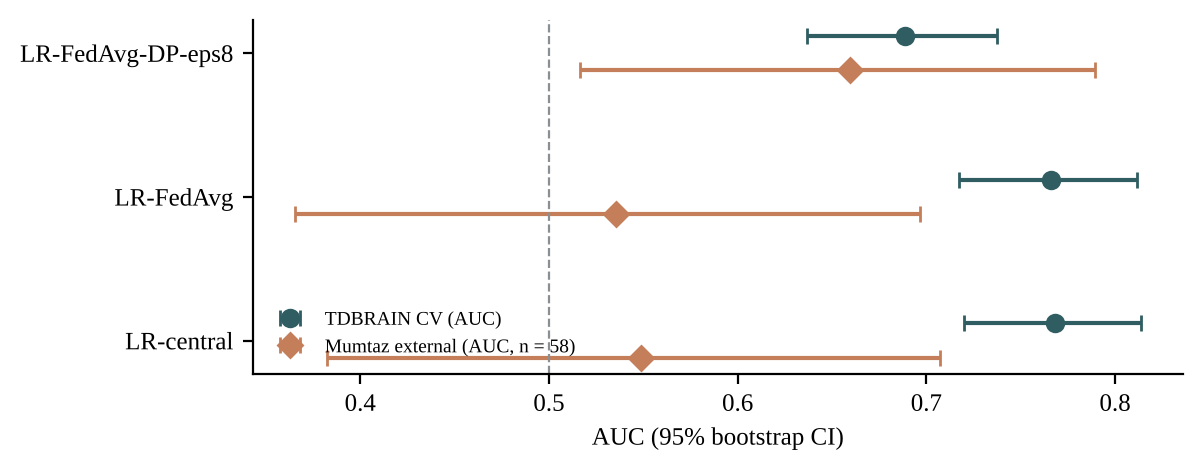
\includegraphics[width=0.85\textwidth]{fig_external.png}
\caption[TDBRAIN cross-validated AUC against Mumtaz external AUC for the same model recipes]{TDBRAIN cross-validated AUC against Mumtaz external AUC for the same model recipes}\label{fig:fig_external}
\end{figure}

\section{Explainability}
Figure~\ref{fig:fig_explain} shows the standardised coefficients of the spectral model, averaged over folds and grouped by band and region, for features whose sign was stable in at least four of five folds. These describe what the model uses on this data set and explain the model, not the disorder: correlated features share weight, and age may be reflected in them.

\begin{figure}[!htbp]\centering
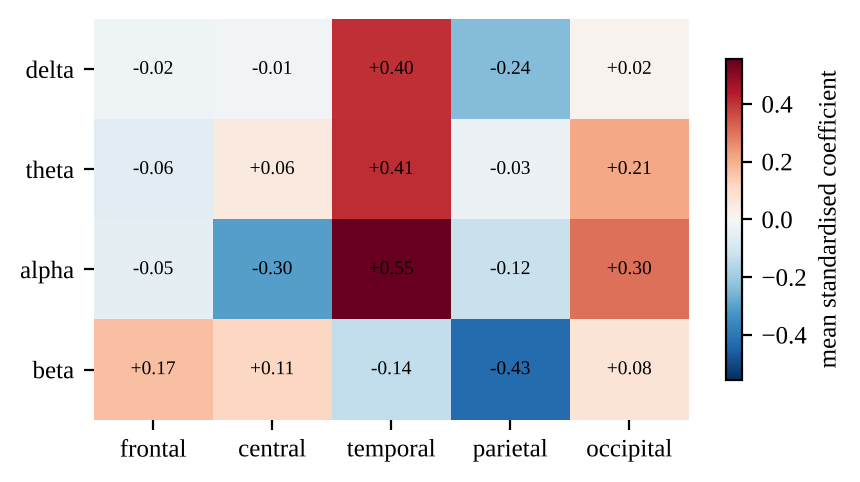
\includegraphics[width=0.70\textwidth]{fig_explain.png}
\caption[Stable logistic-regression coefficients by band and region (explains the model, not the disorder)]{Stable logistic-regression coefficients by band and region (explains the model, not the disorder)}\label{fig:fig_explain}
\end{figure}
The same coefficients drawn on the scalp (Figure~\ref{fig:fig_topo_coef}) show that the model spreads its weight over several regions and bands rather than relying on a single site; filled dots mark channels whose coefficient kept the same sign in at least four of five folds. For the preliminary EEGNet model, the spatial patterns of the depthwise filters (Figure~\ref{fig:fig_eegnet_patterns}) are smooth and broad, as expected from a network that combines all 19 channels in its spatial stage. Because this model was trained on one fold only, its patterns are illustrative.

\begin{figure}[!htbp]\centering
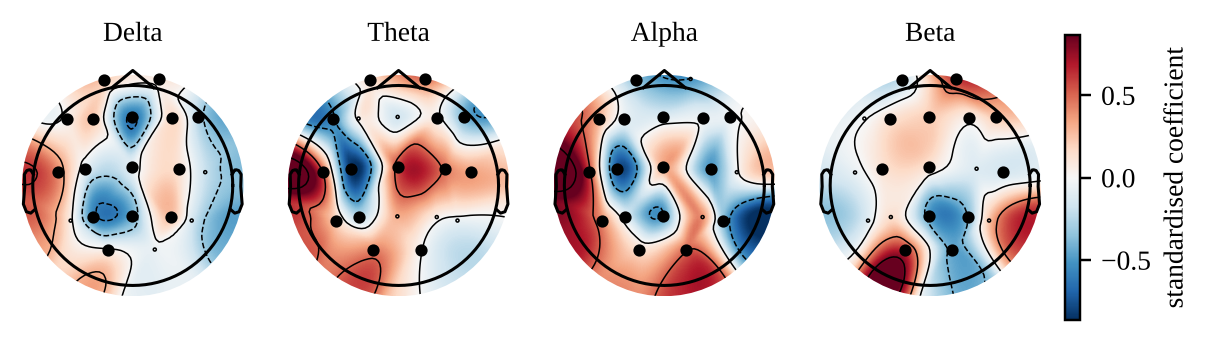
\includegraphics[width=0.98\textwidth]{fig_topo_coef.png}
\caption[Mean standardised logistic-regression coefficient per channel and band; filled dots mark sign-stable channels (explains the model, not the disorder)]{Mean standardised logistic-regression coefficient per channel and band; filled dots mark sign-stable channels (explains the model, not the disorder)}\label{fig:fig_topo_coef}
\end{figure}
\begin{figure}[!htbp]\centering
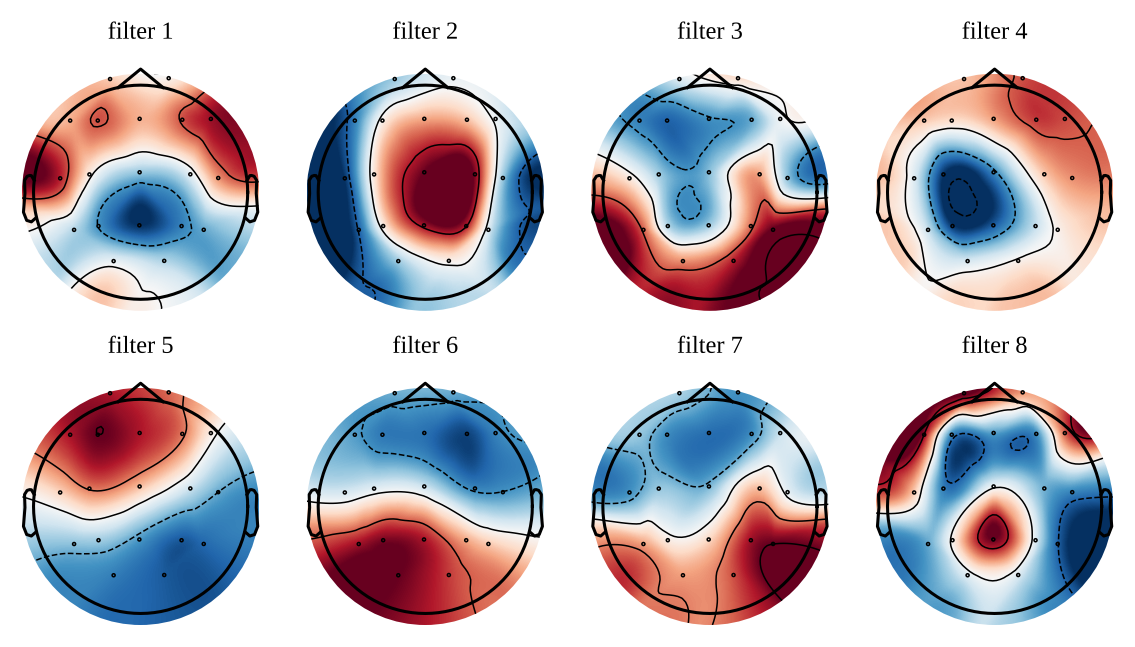
\includegraphics[width=0.80\textwidth]{fig_eegnet_patterns.png}
\caption[Spatial patterns of the eight depthwise filters of the fold-0 EEGNet model (preliminary; explains the model, not the disorder)]{Spatial patterns of the eight depthwise filters of the fold-0 EEGNet model (preliminary; explains the model, not the disorder)}\label{fig:fig_eegnet_patterns}
\end{figure}

\section{Answering the Research Questions}
\begin{table}[!htbp]\centering\small\setstretch{1.1}
\caption{Answers to the research questions from the current evidence}\label{tab:rq}
\begin{tabularx}{\textwidth}{lXl}
\toprule
 & Finding & Present answer\\
\midrule
RQ1 & Spectral LR reached 0.738 BA on T1 under participant-level evaluation; part of this is age. EEGNet did not outperform it on fold 0. & Moderate separation; deep vs features open\\
RQ2 & FedAvg cost 0.034 BA and was robust to skew and dropout; DP cost 0.086--0.112 BA at $\varepsilon$ = 8 to 3. & Federation cheap; DP costs about 0.1\\
RQ3 & LiRA AUC fell from 0.563 to $\approx$ 0.5 with DP. External AUC was near chance and the data sets were separable (probe AUC 0.966). & DP removes measurable leakage; transfer fails\\
\bottomrule
\end{tabularx}
\end{table}

\chapter{Conclusion and Future Work}

\section{Conclusion}
A benchmark that guards against participant leakage was assembled on a large clinical EEG archive and used to quantify what federated and differentially private training cost and what they protect. Its principal results can be summarised as follows:

\begin{enumerate}[leftmargin=1.6em,itemsep=2pt,topsep=2pt]
\item A reproducible pipeline from the TDBRAIN release to frozen participant-level splits and clean epochs, which processed 796 of 806 labelled recordings and passed a shuffled-label leakage control.
\item A spectral baseline with balanced accuracy 0.738 on MDD vs healthy, shown by an age-only control to be partly but not wholly explained by age, and a much weaker separation of MDD from other patients (0.553).
\item Federated training that lost only 0.034 in balanced accuracy and was robust to label skew and client dropout, while single-site training lost 0.099.
\item Participant-level differential privacy that cost about 0.09--0.11 in balanced accuracy and reduced a participant-level membership-inference attack to chance.
\item A one-time external test showing poor transfer to Mumtaz, explained by a near-perfect separation of the two data sets (probe AUC 0.966).
\end{enumerate}
For the linear model the answer is therefore clear: sharing model updates instead of data costs little, protecting each person with DP costs roughly a tenth of balanced accuracy and leaves the attack with no edge, and moving to a different recording site is where performance breaks down. The deep-learning comparison still needs full-scale runs. None of these outputs is intended for diagnosis.


\section{Limitations}
\begin{itemize}[leftmargin=1.6em,itemsep=2pt,topsep=2pt]
\item The simulated clients are random partitions of one archive, not hospitals with different hardware and populations.
\item EEGNet was run only on one fold under a reduced budget; E12, FedProx, FedBN and the ablations were not run.
\item Federated, DP and audit experiments used one seed; the external set is small (58 participants with eyes-closed data).
\item Healthy participants were younger than those with MDD, and age is partly confounded with the label.
\item Medication was not systematically recorded in TDBRAIN, and clinical labels carry noise and comorbidity.
\item The sex coding of the participant table was not confirmed, so sex is reported only as raw codes.
\item This is a research benchmark and not a diagnostic tool.
\end{itemize}

\section{Future Work}
\begin{enumerate}[leftmargin=1.6em,itemsep=2pt,topsep=2pt]
\item \textbf{Complete the deep-learning track.} Run EEGNet under the full specification (5 folds, 3 seeds, up to 100 epochs), with FedProx, FedBN, DP and LiRA, on a machine with a graphics card.
\item \textbf{Run the leakage demonstration and ablations.} E12 (segment split), E14--E20 (channel set, preprocessing, eyes-open, recording length, client number, within-Mumtaz CV).
\item \textbf{Control for age.} Match groups by age or include age as a covariate and repeat the main comparisons.
\item \textbf{Use real sites.} Add de-identified recordings from a second institution, such as AIIMS, after ethics approval, so that clients differ in hardware and population.
\item \textbf{Strengthen privacy.} Add secure aggregation so that the server sees only the sum of client updates.
\item \textbf{Address data-set shift.} Study per-site normalisation and domain adaptation, and test whether they help external transfer without leaking test information.
\end{enumerate}
\begin{figure}[!htbp]\centering
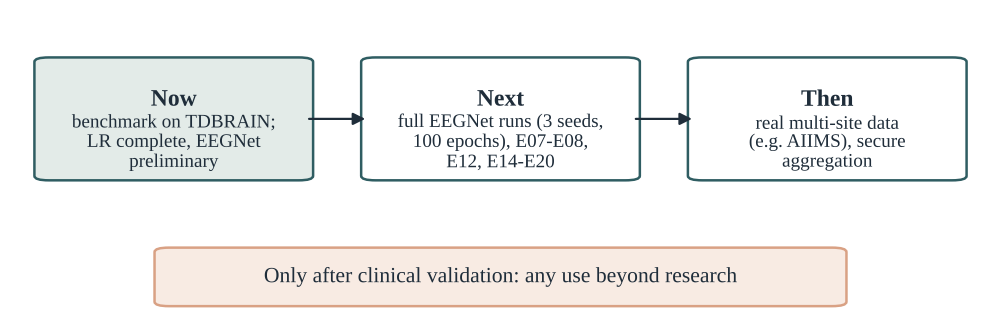
\includegraphics[width=0.90\textwidth]{fig_roadmap.png}
\caption[Roadmap from the current benchmark to multi-site evaluation]{Roadmap from the current benchmark to multi-site evaluation}\label{fig:fig_roadmap}
\end{figure}

\clearpage\phantomsection\addcontentsline{toc}{chapter}{REFERENCES}
\begin{thebibliography}{99}\small\setstretch{1.1}
\bibitem{who} World Health Organization, "Depressive disorder (depression)," Fact sheet, 2023. [Online]. Available: https://www.who.int/news-room/fact-sheets/detail/depression
\bibitem{review} D. de Aguiar Neto and J. L. G. Rosa, "Depression biomarkers using non-invasive EEG: A review," \emph{Neuroscience \& Biobehavioral Reviews}, vol. 105, pp. 83--93, 2019. doi: 10.1016/j.neubiorev.2019.07.021.
\bibitem{leak} G. Brookshire \emph{et al.}, "Data leakage in deep learning studies of translational EEG," \emph{Frontiers in Neuroscience}, vol. 18, art. 1373515, 2024. doi: 10.3389/fnins.2024.1373515.
\bibitem{kaissis} G. A. Kaissis, M. R. Makowski, D. Rückert and R. F. Braren, "Secure, privacy-preserving and federated machine learning in medical imaging," \emph{Nature Machine Intelligence}, vol. 2, pp. 305--311, 2020. doi: 10.1038/s42256-020-0186-1.
\bibitem{fedavg} B. McMahan, E. Moore, D. Ramage, S. Hampson and B. Agüera y Arcas, "Communication-efficient learning of deep networks from decentralized data," in \emph{Proc. 20th Int. Conf. Artificial Intelligence and Statistics (AISTATS)}, PMLR vol. 54, 2017, pp. 1273--1282.
\bibitem{dwork} C. Dwork and A. Roth, "The algorithmic foundations of differential privacy," \emph{Foundations and Trends in Theoretical Computer Science}, vol. 9, no. 3--4, pp. 211--407, 2014.
\bibitem{tdbrain} H. van Dijk \emph{et al.}, "The two decades brainclinics research archive for insights in neurophysiology (TDBRAIN) database," \emph{Scientific Data}, vol. 9, art. 333, 2022. doi: 10.1038/s41597-022-01409-z.
\bibitem{faa} A. G. van der Vinne, F. Wiersma, M. Arns \emph{et al.}, "Frontal alpha asymmetry as a diagnostic marker in depression: Fact or fiction? A meta-analysis," \emph{NeuroImage: Clinical}, vol. 16, pp. 79--87, 2017. doi: 10.1016/j.nicl.2017.07.006.
\bibitem{mumtaz17} W. Mumtaz, L. Xia, S. S. A. Ali, M. A. M. Yasin, M. Hussain and A. S. Malik, "Electroencephalogram (EEG)-based computer-aided technique to diagnose major depressive disorder (MDD)," \emph{Biomedical Signal Processing and Control}, vol. 31, pp. 108--115, 2017. doi: 10.1016/j.bspc.2016.07.006.
\bibitem{mumtazdata} W. Mumtaz, "MDD patients and healthy controls EEG data (new)," figshare, 2016. doi: 10.6084/m9.figshare.4244171.
\bibitem{varo} G. Varoquaux, "Cross-validation failure: Small sample sizes lead to large error bars," \emph{NeuroImage}, vol. 180, pp. 68--77, 2018. doi: 10.1016/j.neuroimage.2017.06.061.
\bibitem{fedprox} T. Li, A. K. Sahu, M. Zaheer, M. Sanjabi, A. Talwalkar and V. Smith, "Federated optimization in heterogeneous networks," in \emph{Proc. Machine Learning and Systems}, vol. 2, 2020, pp. 429--450.
\bibitem{fedbn} X. Li, M. Jiang, X. Zhang, M. Kamp and Q. Dou, "FedBN: Federated learning on non-IID features via local batch normalization," in \emph{Proc. International Conference on Learning Representations (ICLR)}, 2021.
\bibitem{rieke} N. Rieke \emph{et al.}, "The future of digital health with federated learning," \emph{npj Digital Medicine}, vol. 3, art. 119, 2020. doi: 10.1038/s41746-020-00323-1.
\bibitem{dlg} L. Zhu, Z. Liu and S. Han, "Deep leakage from gradients," in \emph{Advances in Neural Information Processing Systems}, vol. 32, 2019.
\bibitem{abadi} M. Abadi \emph{et al.}, "Deep learning with differential privacy," in \emph{Proc. ACM SIGSAC Conference on Computer and Communications Security (CCS)}, 2016, pp. 308--318. doi: 10.1145/2976749.2978318.
\bibitem{rdp} I. Mironov, "Rényi differential privacy," in \emph{Proc. IEEE 30th Computer Security Foundations Symposium (CSF)}, 2017, pp. 263--275. doi: 10.1109/CSF.2017.11.
\bibitem{balle} B. Balle, G. Barthe, M. Gaboardi, J. Hsu and T. Sato, "Hypothesis testing interpretations and Rényi differential privacy," in \emph{Proc. 23rd Int. Conf. Artificial Intelligence and Statistics (AISTATS)}, PMLR vol. 108, 2020, pp. 2496--2506.
\bibitem{userdp} H. B. McMahan, D. Ramage, K. Talwar and L. Zhang, "Learning differentially private recurrent language models," in \emph{Proc. International Conference on Learning Representations (ICLR)}, 2018.
\bibitem{shokri} R. Shokri, M. Stronati, C. Song and V. Shmatikov, "Membership inference attacks against machine learning models," in \emph{Proc. IEEE Symposium on Security and Privacy}, 2017, pp. 3--18. doi: 10.1109/SP.2017.41.
\bibitem{lira} N. Carlini, S. Chien, M. Nasr, S. Song, A. Terzis and F. Tramèr, "Membership inference attacks from first principles," in \emph{Proc. IEEE Symposium on Security and Privacy}, 2022, pp. 1897--1914. doi: 10.1109/SP46214.2022.9833649.
\bibitem{welch} P. Welch, "The use of fast Fourier transform for the estimation of power spectra," \emph{IEEE Trans. Audio and Electroacoustics}, vol. 15, no. 2, pp. 70--73, 1967. doi: 10.1109/TAU.1967.1161901.
\bibitem{sklearn} F. Pedregosa \emph{et al.}, "Scikit-learn: Machine learning in Python," \emph{Journal of Machine Learning Research}, vol. 12, pp. 2825--2830, 2011.
\bibitem{eegnet} V. J. Lawhern \emph{et al.}, "EEGNet: a compact convolutional neural network for EEG-based brain--computer interfaces," \emph{Journal of Neural Engineering}, vol. 15, art. 056013, 2018. doi: 10.1088/1741-2552/aace8c.
\bibitem{gn} Y. Wu and K. He, "Group normalization," in \emph{Proc. European Conference on Computer Vision (ECCV)}, 2018, pp. 3--19.
\bibitem{adam} D. P. Kingma and J. Ba, "Adam: A method for stochastic optimization," in \emph{Proc. International Conference on Learning Representations (ICLR)}, 2015.
\bibitem{flower} D. J. Beutel \emph{et al.}, "Flower: A friendly federated learning research framework," arXiv:2007.14390, 2020.
\bibitem{opacus} A. Yousefpour \emph{et al.}, "Opacus: User-friendly differential privacy library in PyTorch," arXiv:2109.12298, 2021.
\bibitem{boot} B. Efron and R. J. Tibshirani, \emph{An Introduction to the Bootstrap}. New York: Chapman \& Hall, 1993.
\bibitem{mne} A. Gramfort \emph{et al.}, "MEG and EEG data analysis with MNE-Python," \emph{Frontiers in Neuroscience}, vol. 7, art. 267, 2013. doi: 10.3389/fnins.2013.00267.
\bibitem{torch} A. Paszke \emph{et al.}, "PyTorch: An imperative style, high-performance deep learning library," in \emph{Advances in Neural Information Processing Systems}, vol. 32, 2019.
\bibitem{mlflow} M. Zaharia \emph{et al.}, "Accelerating the machine learning lifecycle with MLflow," \emph{IEEE Data Engineering Bulletin}, vol. 41, no. 4, pp. 39--45, 2018.
\end{thebibliography}
\end{document}
